\documentclass[journal]{IEEEtran}
\usepackage[a5paper, margin=10mm]{geometry}
%\usepackage{lmodern} % Ensure lmodern is loaded for pdflatex
\usepackage{tfrupee}

\setlength{\headheight}{1cm}
\setlength{\headsep}{0mm}

\usepackage{gvv-book}
\usepackage{gvv}
\usepackage{amsfonts}

\hypersetup{
    colorlinks=true,
    urlcolor=black
}

\makeindex

\begin{document}

\bibliographystyle{IEEEtran}
\onecolumn

\title{
\begin{center}
RGB to Black and White: A Clear Journey
\\
\rule{0.8\columnwidth}{0.6pt}
\end{center}
}

\author{
    \vspace{11cm}
    \begin{center}
        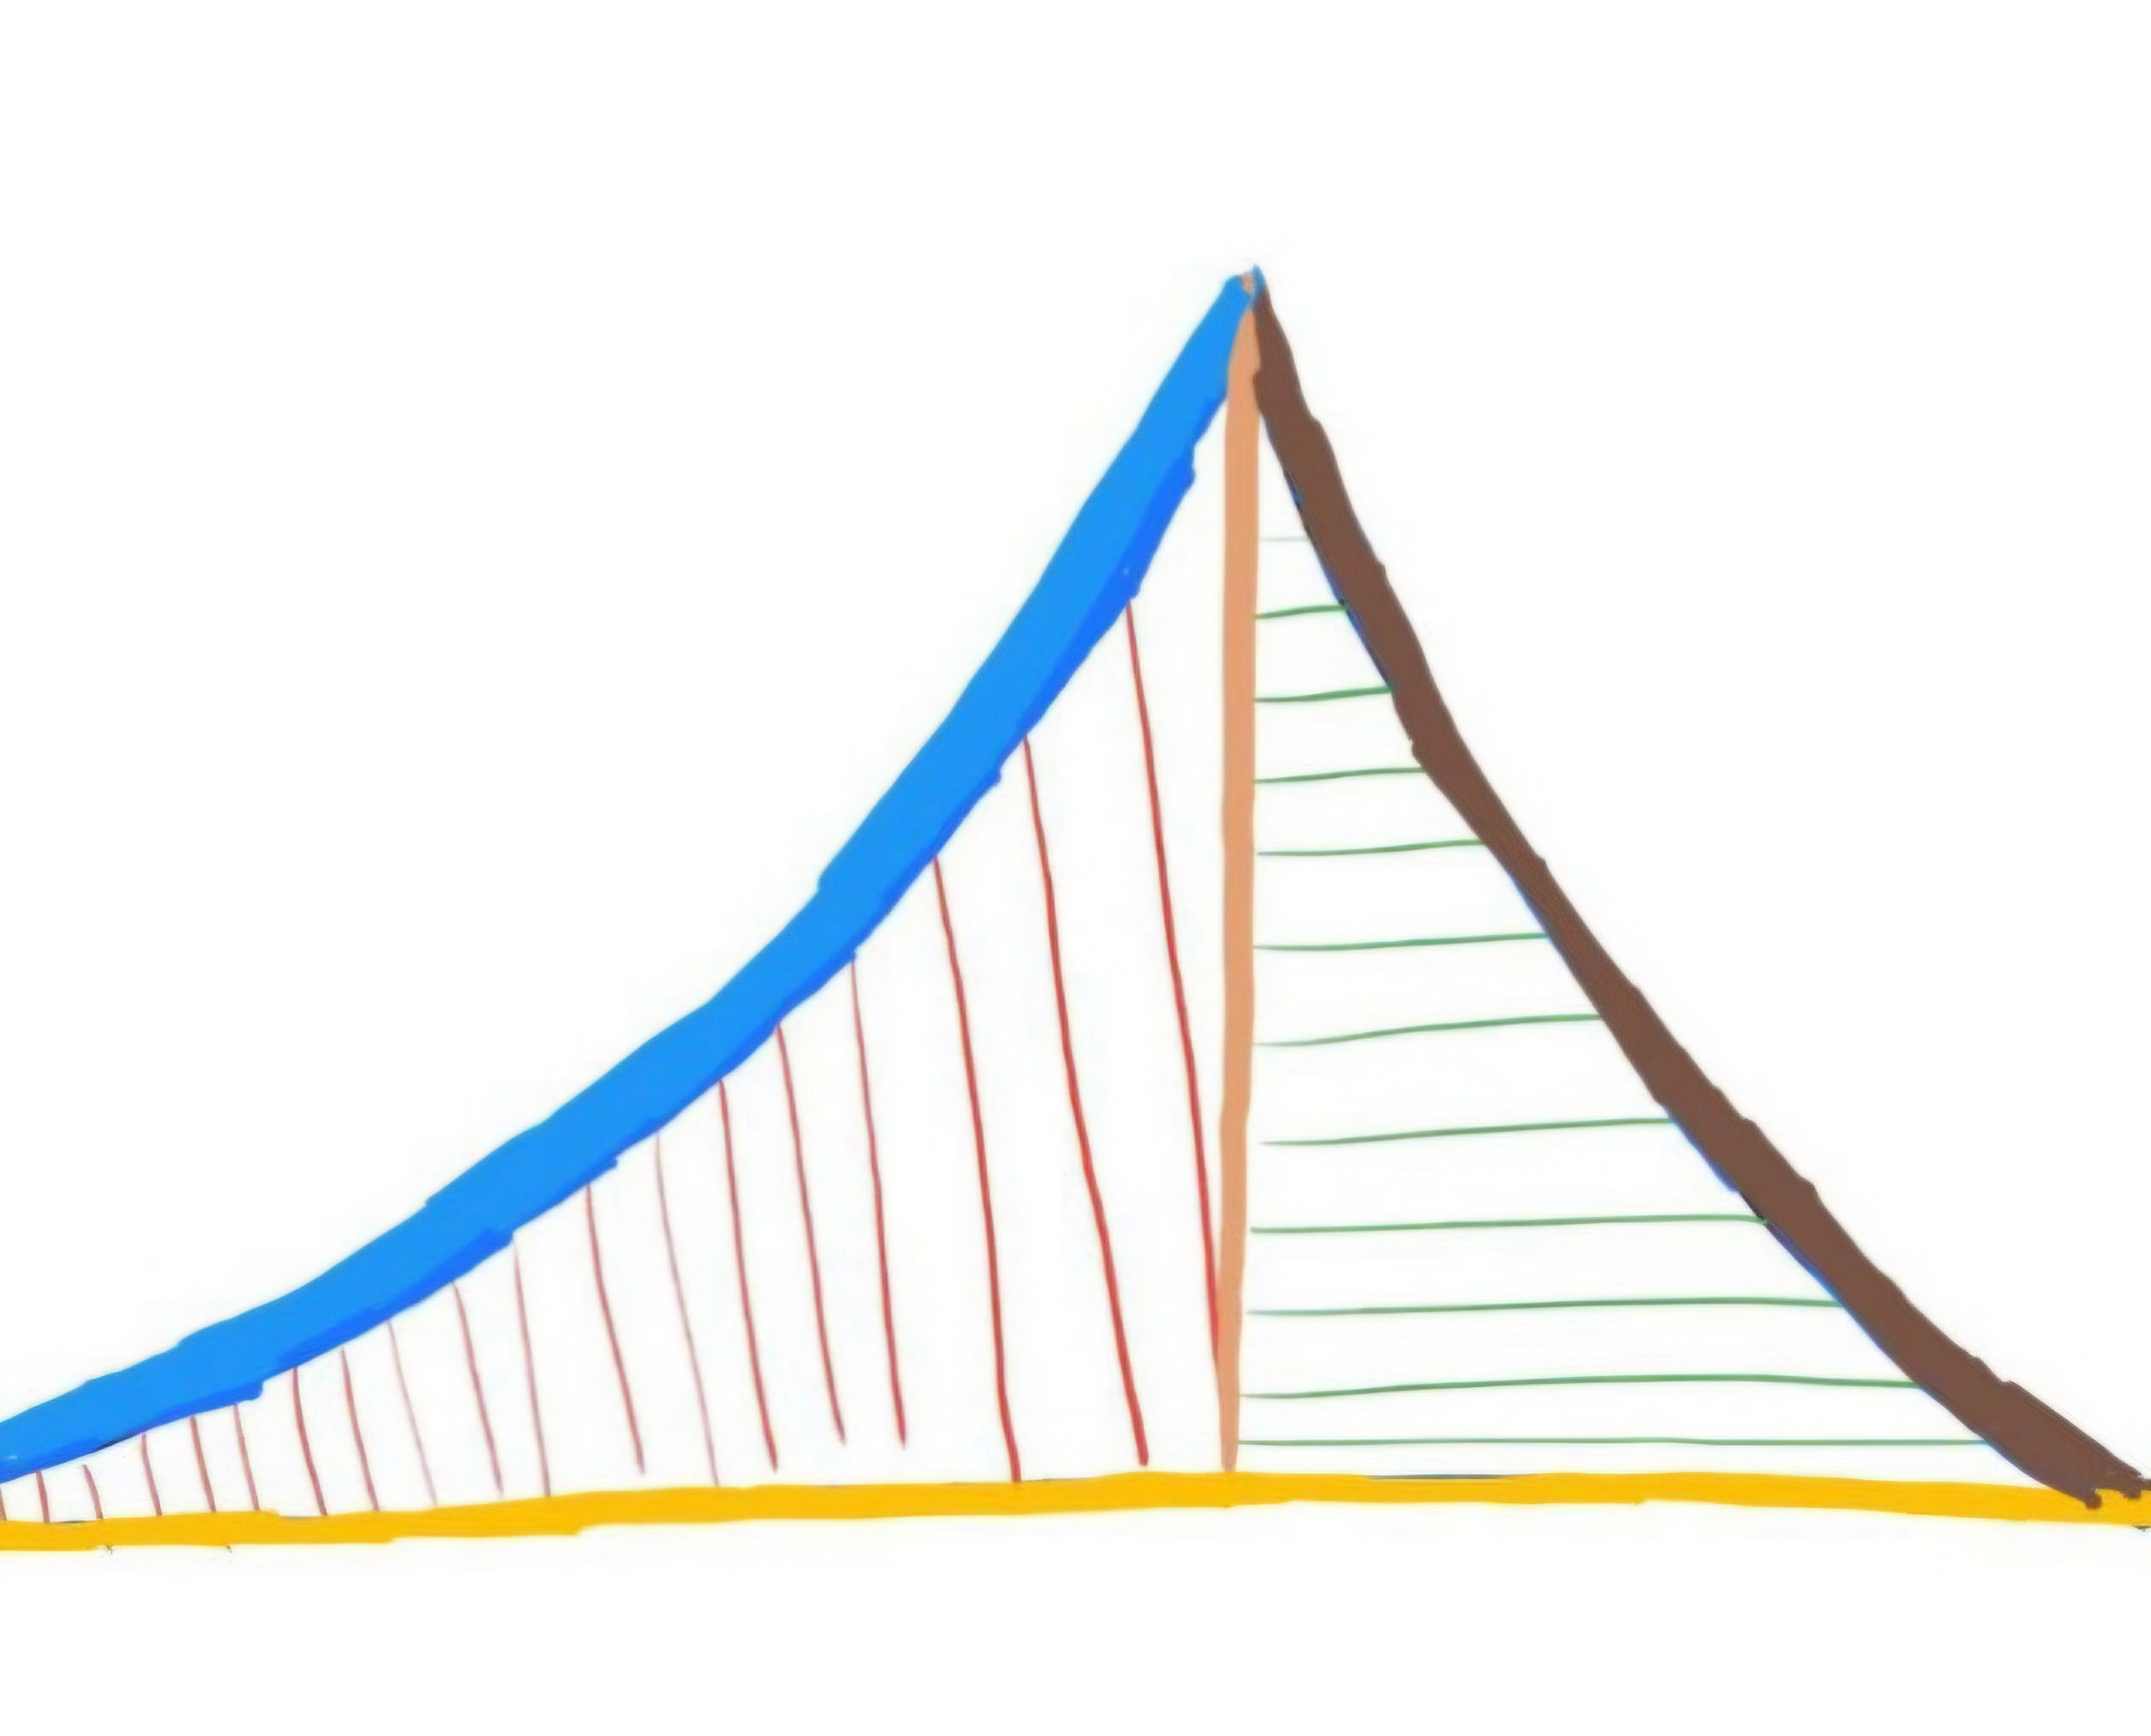
\includegraphics[width=0.2\columnwidth]{figs/logo.jpg}
        \\
        {\huge G. V. V. Sharma}
    \end{center}
}

\maketitle

\newpage
\section*{About this Article}
This article is written by T. P. Siddardha Reddy under the guidance
of Dr. GVV Sharma, an Associate Professor in IITH EE Department.

This article presents a clear journey from a coloured RGB image to a
black-and-white representation. The objective is to understand the
representation of RGB image data, the storage of raw bitmap data, the
role of colour conversion, and the reduction of colour information to
intensity information.

The presentation follows the style used throughout Dr GVV Sharma's documents:
definitions and formulae are introduced first, followed by the
conversion procedure, clustering methods, implementation, and output.
The mathematical expressions are kept explicit so that the complete
conversion can be followed from the original RGB values to the final
black-and-white image.

Github: https://github.com/gadepall/
\\
License: https://creativecommons.org/licenses/by-sa/3.0/
\\
Published on: 3rd October 2026


\newpage
\tableofcontents

\newpage
\onecolumn

\setcounter{secnumdepth}{2}

\renewcommand{\thesection}{\arabic{section}}
\renewcommand{\thesubsection}{\thesection.\arabic{subsection}}
\renewcommand{\thesubsectiondis}{\thesubsection.}

\renewcommand{\theequation}{\thesubsection.\arabic{equation}}
\numberwithin{equation}{subsection}
\numberwithin{figure}{section}
\numberwithin{table}{section}

% Chapter 1 starts at the top of the page
\section{\textbf{Introduction}}
\subsection{RGB Image}

An RGB image represents colour using three components: Red, Green, and
Blue. A pixel can therefore be represented by the tuple
\begin{align}
P_{ij} &= (R_{ij},G_{ij},B_{ij})\label{eq:rgb_pixel}
\end{align}

For a conventional 8-bit RGB image, each component is represented using
8 bits. Hence, one pixel requires
\begin{align}
8+8+8 &= 24\label{eq:rgb_bits}
\end{align}
bits of colour information.

For an image containing $M\times N$ pixels, the image may be viewed as
three matrices,
\begin{align}
R&\in\mathbb{R}^{M\times N}\label{eq:r_matrix}\\
G&\in\mathbb{R}^{M\times N}\label{eq:g_matrix}\\
B&\in\mathbb{R}^{M\times N}\label{eq:b_matrix}
\end{align}

The conversion to black and white is therefore a reduction from three
colour values per pixel to one intensity value per pixel.


\vspace*{5\baselineskip}
\section{\textbf{RGB Image Representation}}
\subsection{RGB Pixel Representation}

The three components of an RGB pixel are normally represented in the
range $0$ to $255$ for an 8-bit image:
\begin{align}
0\leq R,G,B\leq255\label{eq:rgb_range}
\end{align}

The pixel at position $(i,j)$ is
\begin{align}
P_{ij}=(R_{ij},G_{ij},B_{ij})\label{eq:rgb_tuple}
\end{align}
\vspace*{\baselineskip}
\subsection{Colour Information}

Different RGB tuples may produce colours having similar perceived
brightness. Consequently, choosing only one RGB component would discard
important information. A weighted combination is therefore used when
the objective is to obtain grayscale intensity.


\vspace*{5\baselineskip}
\section{\textbf{Raw Bitmap and JPEG Representation}}
\subsection{Raw Bitmap Representation}

A raw RGB bitmap stores the colour components of the pixels directly.
For a $2\times2$ group of pixels,
\begin{align}
\begin{bmatrix}
(R_{11},G_{11},B_{11}) & (R_{12},G_{12},B_{12})\\
(R_{21},G_{21},B_{21}) & (R_{22},G_{22},B_{22})
\end{bmatrix}\label{eq:raw_rgb_2x2}
\end{align}

\vspace*{\baselineskip}

\subsection{JPEG Representation}

JPEG uses a transformed and compressed representation rather than
storing every RGB tuple independently. The JPEG standard defines processes
for converting source image data to compressed image data.

The common colour information is calculated, and the formulae used for
this conversion are listed in the next section.

\vspace*{\baselineskip}

\subsection{Per-Pixel Storage}

For an image containing $N$ pixels, an 8-bit RGB representation requires
three separate 8-bit colour components for every pixel. Hence, the raw
colour information requires
\begin{align}
3\times8N&=24N\label{eq:rgb_storage_bits}
\end{align}
bits.

If the image is converted directly from RGB to grayscale, only the
luminance value $Y$ is retained for each pixel. With an 8-bit grayscale
representation, this requires
\begin{align}
1\times8N&=8N\label{eq:grayscale_storage_bits}
\end{align}
bits.

Thus, the storage changes from $24N$ bits for RGB to $8N$ bits for
grayscale. The storage ratio is therefore
\begin{align}
\frac{8N}{24N}&=\frac{1}{3}\label{eq:rgb_grayscale_ratio}
\end{align}
so the grayscale representation requires one-third of the raw RGB
storage, corresponding to a reduction of two-thirds.

When the image is represented using $Y$, $Cb$, and $Cr$, the three
components are still separate components. Each component is normally
represented using 8-bit samples; the reduction in storage can instead be
obtained by reducing the spatial sampling of the chrominance components.
In particular, with 4:2:0 chroma subsampling, the $Y$ component retains
$N$ samples, while $Cb$ and $Cr$ each contain $N/4$ samples.

Therefore, before the additional JPEG transform and coding stages, the
sample storage can be written as
\begin{align}
8N+8\frac{N}{4}+8\frac{N}{4}
&=12N\label{eq:ycbcr_420_storage_bits}
\end{align}
bits.

Thus, the factor of four applies to the \emph{number of chrominance
samples}, not to the number of bits in an individual $Cb$ or $Cr$ sample.
The $Y$ component is retained at full spatial resolution because it carries
the intensity information for every pixel.

For example, in a $2\times2$ group containing four $Y$ samples, 4:2:0
subsampling uses one $Cb$ sample and one $Cr$ sample for the group. The
$Cb$ and $Cr$ samples are therefore stored separately, but they are shared
spatially by the four corresponding pixels.

The comparison above describes sample storage before the main JPEG
compression stages. The actual size of a JPEG file is different because
JPEG additionally uses transformation, quantisation, and entropy coding
as part of its coding process.


\vspace*{5\baselineskip}
\section{\textbf{Colour Conversion}}
\subsection{RGB to Luminance and Chrominance}

The RGB components may be transformed into three separate components,
luminance $Y$ and chrominance $Cb$ and $Cr$:
\begin{align}
Y  &= 0.299R + 0.587G + 0.114B\label{eq:y_luminance}\\
Cb &= -0.168736R - 0.331264G + 0.5B + 128\label{eq:cb_chrominance}\\
Cr &= 0.5R - 0.418688G - 0.081312B + 128\label{eq:cr_chrominance}
\end{align}

Here, $Y$ represents luminance, while $Cb$ and $Cr$ represent
chrominance information. The $Cb$ and $Cr$ components carry colour-difference
information associated with blue and red, respectively. They are separate
8-bit components in the usual 8-bit representation; they are not single-bit
colour indicators.
\vspace*{\baselineskip}
\subsection{Chrominance Components}

The $Cb$ component describes the blue-related colour difference and
$Cr$ describes the red-related colour difference. These components
retain colour information that is not required when only grayscale
intensity is required.

When chroma subsampling is used, the $Cb$ and $Cr$ components can be
stored at a lower spatial sampling rate than $Y$. For example, in 4:2:0
subsampling, each $2\times2$ group of pixels retains four $Y$ samples but
uses one $Cb$ sample and one $Cr$ sample. Thus, the chrominance components
remain separate components, while fewer chrominance samples are stored.
\vspace*{\baselineskip}
\subsection{Luminance Weighting}

The coefficients in the luminance equation are different because the
human visual system does not perceive the three RGB components with
 equal sensitivity:
\begin{align}
0.587&>0.299>0.114\label{eq:luminance_weights}
\end{align}

The green component consequently has the largest contribution to
luminance, followed by red and then blue.
\vspace*{\baselineskip}
\subsection{Information Reduction}

For the purpose of grayscale conversion, the colour pixel $(R,G,B)$ is
reduced to the single luminance value $Y$. The $Cb$ and $Cr$ components
carry the colour-difference information and are therefore not required
for the final grayscale intensity image.


\vspace*{5\baselineskip}
\section{\textbf{RGB to Grayscale Conversion}}
\subsection{Grayscale Intensity}

A grayscale image represents every pixel using a single intensity
value:
\begin{align}
Y&=0.299R+0.587G+0.114B\label{eq:grayscale_y}
\end{align}

A small value of $Y$ represents a dark pixel, while a large value
represents a bright pixel.
\vspace*{\baselineskip}
\subsection{Black and White}

A grayscale image contains many intensity levels between black and
white. A black-and-white image instead contains two classes.

Let $T$ denote the selected threshold:
\begin{align}
B(i,j)=
\begin{cases}
0, & Y(i,j)<T,\\
255, & Y(i,j)\geq T.
\end{cases}\label{eq:bw_threshold}
\end{align}

Thus the grayscale intensity is mapped to one of two output values.


\vspace*{5\baselineskip}
\section{\textbf{Grayscale and Black-and-White Conversion Algorithm}}
\subsection{RGB to Grayscale Algorithm}

The conversion procedure is carried out pixel by pixel.

\begin{enumerate}
\item Read the RGB input image.
\item Obtain $R$, $G$, and $B$ for each pixel.
\item Calculate the luminance $Y$.
\item Store $Y$ as the grayscale intensity.
\item Select the threshold $T$.
\item Compare every grayscale value with $T$.
\item Assign black or white according to the threshold condition.
\item Save the resulting image.
\end{enumerate}

The complete transformation is
\begin{align}
RGB &\rightarrow Y \rightarrow \text{Threshold}
\rightarrow \text{Black/White}\label{eq:rgb_bw_pipeline}
\end{align}
\vspace*{\baselineskip}
\subsection{Mapping to the Output Image}

The calculated intensity matrix is passed to the image-writing stage.
When JPEG is selected, the image-writing stage performs the
corresponding JPEG encoding and compression.


\vspace*{5\baselineskip}
\section{\textbf{Clustering Methods and Analysis}}
\subsection{Global Mean Thresholding}

The first dynamic method calculates one reference intensity from the
complete grayscale image. If the grayscale matrix is denoted by $Y$,
the reference is the mean intensity of all pixels:
\begin{align}
\mu &= \frac{1}{MN}\sum_{i=1}^{M}\sum_{j=1}^{N}Y(i,j)\label{eq:global_mean}
\end{align}

Every pixel is then compared with this single image-wide reference. The
corresponding binary decision is
\begin{align}
B(i,j)&=
\begin{cases}
255, & Y(i,j)\geq\mu,\\
0, & Y(i,j)<\mu.
\end{cases}\label{eq:global_mean_threshold}
\end{align}

This method is adaptive in the sense that the reference changes with the
input image, but the reference itself is global. It therefore does not
change from one location to another within the same image.
\vspace*{\baselineskip}
\subsection{Static Reference Thresholding}

For comparison, a fixed reference of $128$ is used in the static
thresholding method. A grayscale pixel is assigned to white when its
intensity is at least $128$ and to black otherwise:
\begin{align}
B(i,j)&=
\begin{cases}
255, & Y(i,j)\geq128,\\
0, & Y(i,j)<128.
\end{cases}\label{eq:static_threshold}
\end{align}

The purpose of this fixed reference is to provide a simple baseline
against which the dynamically calculated references can be compared.
\vspace*{\baselineskip}
\subsection{Gaussian-Weighted Local Reference}

A more localized reference is obtained by applying a Gaussian filter to
the grayscale intensity matrix. Instead of giving every neighbouring
pixel equal importance, the Gaussian function gives greater importance
to pixels close to the point being considered and progressively less
importance to pixels farther away.

The Gaussian weighting function is
\begin{align}
w(d)&=\exp\left(-\frac{d^2}{2\sigma^2}\right)\label{eq:gaussian_weight}
\end{align}

Here, $d$ is the distance from the point being processed and $\sigma$
controls the spatial spread of the Gaussian weighting. The corresponding
local reference can be understood as the weighted average
\begin{align}
\mu_G(i,j)&=
\frac{\displaystyle\sum_{(u,v)\in\mathcal{N}}
w(d_{uv})Y(u,v)}
{\displaystyle\sum_{(u,v)\in\mathcal{N}}w(d_{uv})}\label{eq:gaussian_local_mean}
\end{align}

Thus, the reference intensity is different at different locations in
the image and follows the local intensity distribution smoothly.

In the implementation, this operation is performed using
\texttt{gaussian\_filter}:
\newpage
\begin{lstlisting}[frame=single, basicstyle=\rmfamily]
local_mean = gaussian_filter(
    grayscale_matrix.astype(np.float32), sigma=sigma
)
\end{lstlisting}
\vspace*{\baselineskip}
\subsection{Importance of $\sigma$}

The value of $\sigma$ determines how localized the Gaussian reference
is. A smaller value concentrates the weighting around the current pixel,
so the reference responds strongly to nearby intensity variations. A
larger value spreads the weighting over a wider region, causing pixels
farther from the current point to contribute more significantly.

Consequently, $\sigma=10$ gives the localized reference used in this
implementation, whereas $\sigma=20$ gives the wider reference. As
$\sigma$ becomes sufficiently large, the Gaussian weights over the
relevant region become increasingly similar. The Gaussian-weighted
average therefore approaches the behaviour of an ordinary average over a
broad neighbourhood.
\vspace*{\baselineskip}
\subsection{Purpose of $C=3$}

After the Gaussian local reference is calculated, the implementation
uses the threshold
\begin{align}
T_G(i,j)&=\mu_G(i,j)-C\label{eq:gaussian_threshold}
\end{align}

The constant $C=3$ is introduced as a small offset to the Gaussian local
reference. Subtracting this value slightly lowers the local threshold,
allowing pixels that are marginally darker than the calculated local mean
to still be classified as white. In this implementation, $C=3$ is used
as a small empirical adjustment to fine-tune the sensitivity of the
resulting black-and-white output.
\vspace*{\baselineskip}
\subsection{Gaussian Local Thresholding}

The complete decision made by the Gaussian method is therefore
\begin{align}
B(i,j)&=
\begin{cases}
255, & Y(i,j)\geq\mu_G(i,j)-3,\\
0, & Y(i,j)<\mu_G(i,j)-3.
\end{cases}\label{eq:gaussian_bw_threshold}
\end{align}

The important difference from the global methods is that $\mu_G(i,j)$
is not one constant for the entire image. It is a spatially varying
reference calculated from the surrounding grayscale intensities.
\vspace*{\baselineskip}
\subsection{Computational Consideration}

The Gaussian method provides a locally varying reference, but this comes
at an increased computational cost compared with a single global mean.
Conceptually, the local reference has to be evaluated throughout the
image by considering the surrounding pixels and their Gaussian
contributions. The process can therefore be viewed as
\begin{align}
\text{pixel}\;\rightarrow\;\text{neighbourhood}
\;\rightarrow\;\text{Gaussian weights}
\;\rightarrow\;\text{local reference}
\;\rightarrow\;\text{threshold}\label{eq:gaussian_pipeline}
\end{align}

A larger effective Gaussian neighbourhood also involves a broader set
of surrounding pixels. Thus, although the Gaussian reference provides
better spatial adaptation, a direct pixel-by-pixel implementation can be
time-consuming. The \texttt{scipy.ndimage.gaussian\_filter} function used
here performs the filtering efficiently while implementing the same
Gaussian smoothing principle.


\vspace*{5\baselineskip}

\section{\textbf{Implementation and Output}}
\subsection{Implementation}

The implementation reads an RGB JPEG image and converts the RGB matrix
to a YCbCr representation. The $Y$ component is then retained as the
grayscale intensity matrix. From this grayscale matrix, three different
reference strategies are tested: a fixed reference of $128$, a global
mean reference, and Gaussian local references with two different values of $\sigma$ .\newline
The purpose of taking two differet scenarios is to clearly illustrate that the mode of clustering and averaging chosen depends on the type of image. For Example images with simple graphic arts prefer gaussian but those with complex graphics or natural photos work well with the global average referencing.\newline
Hence we have to use some machone learning algorithms and models so they can be trained with the data available about best referencing based on the situation, which will be used by them further for a new situation, and this implementation is beyond the scope of this article.
\vspace*{\baselineskip}
\subsection{Testing Case 1: Scenery}

The first test case uses a scenery image. The outputs are presented in
the following order so that the effect of each reference method can be
compared with the original image.

\begin{figure}[H]
    \centering
    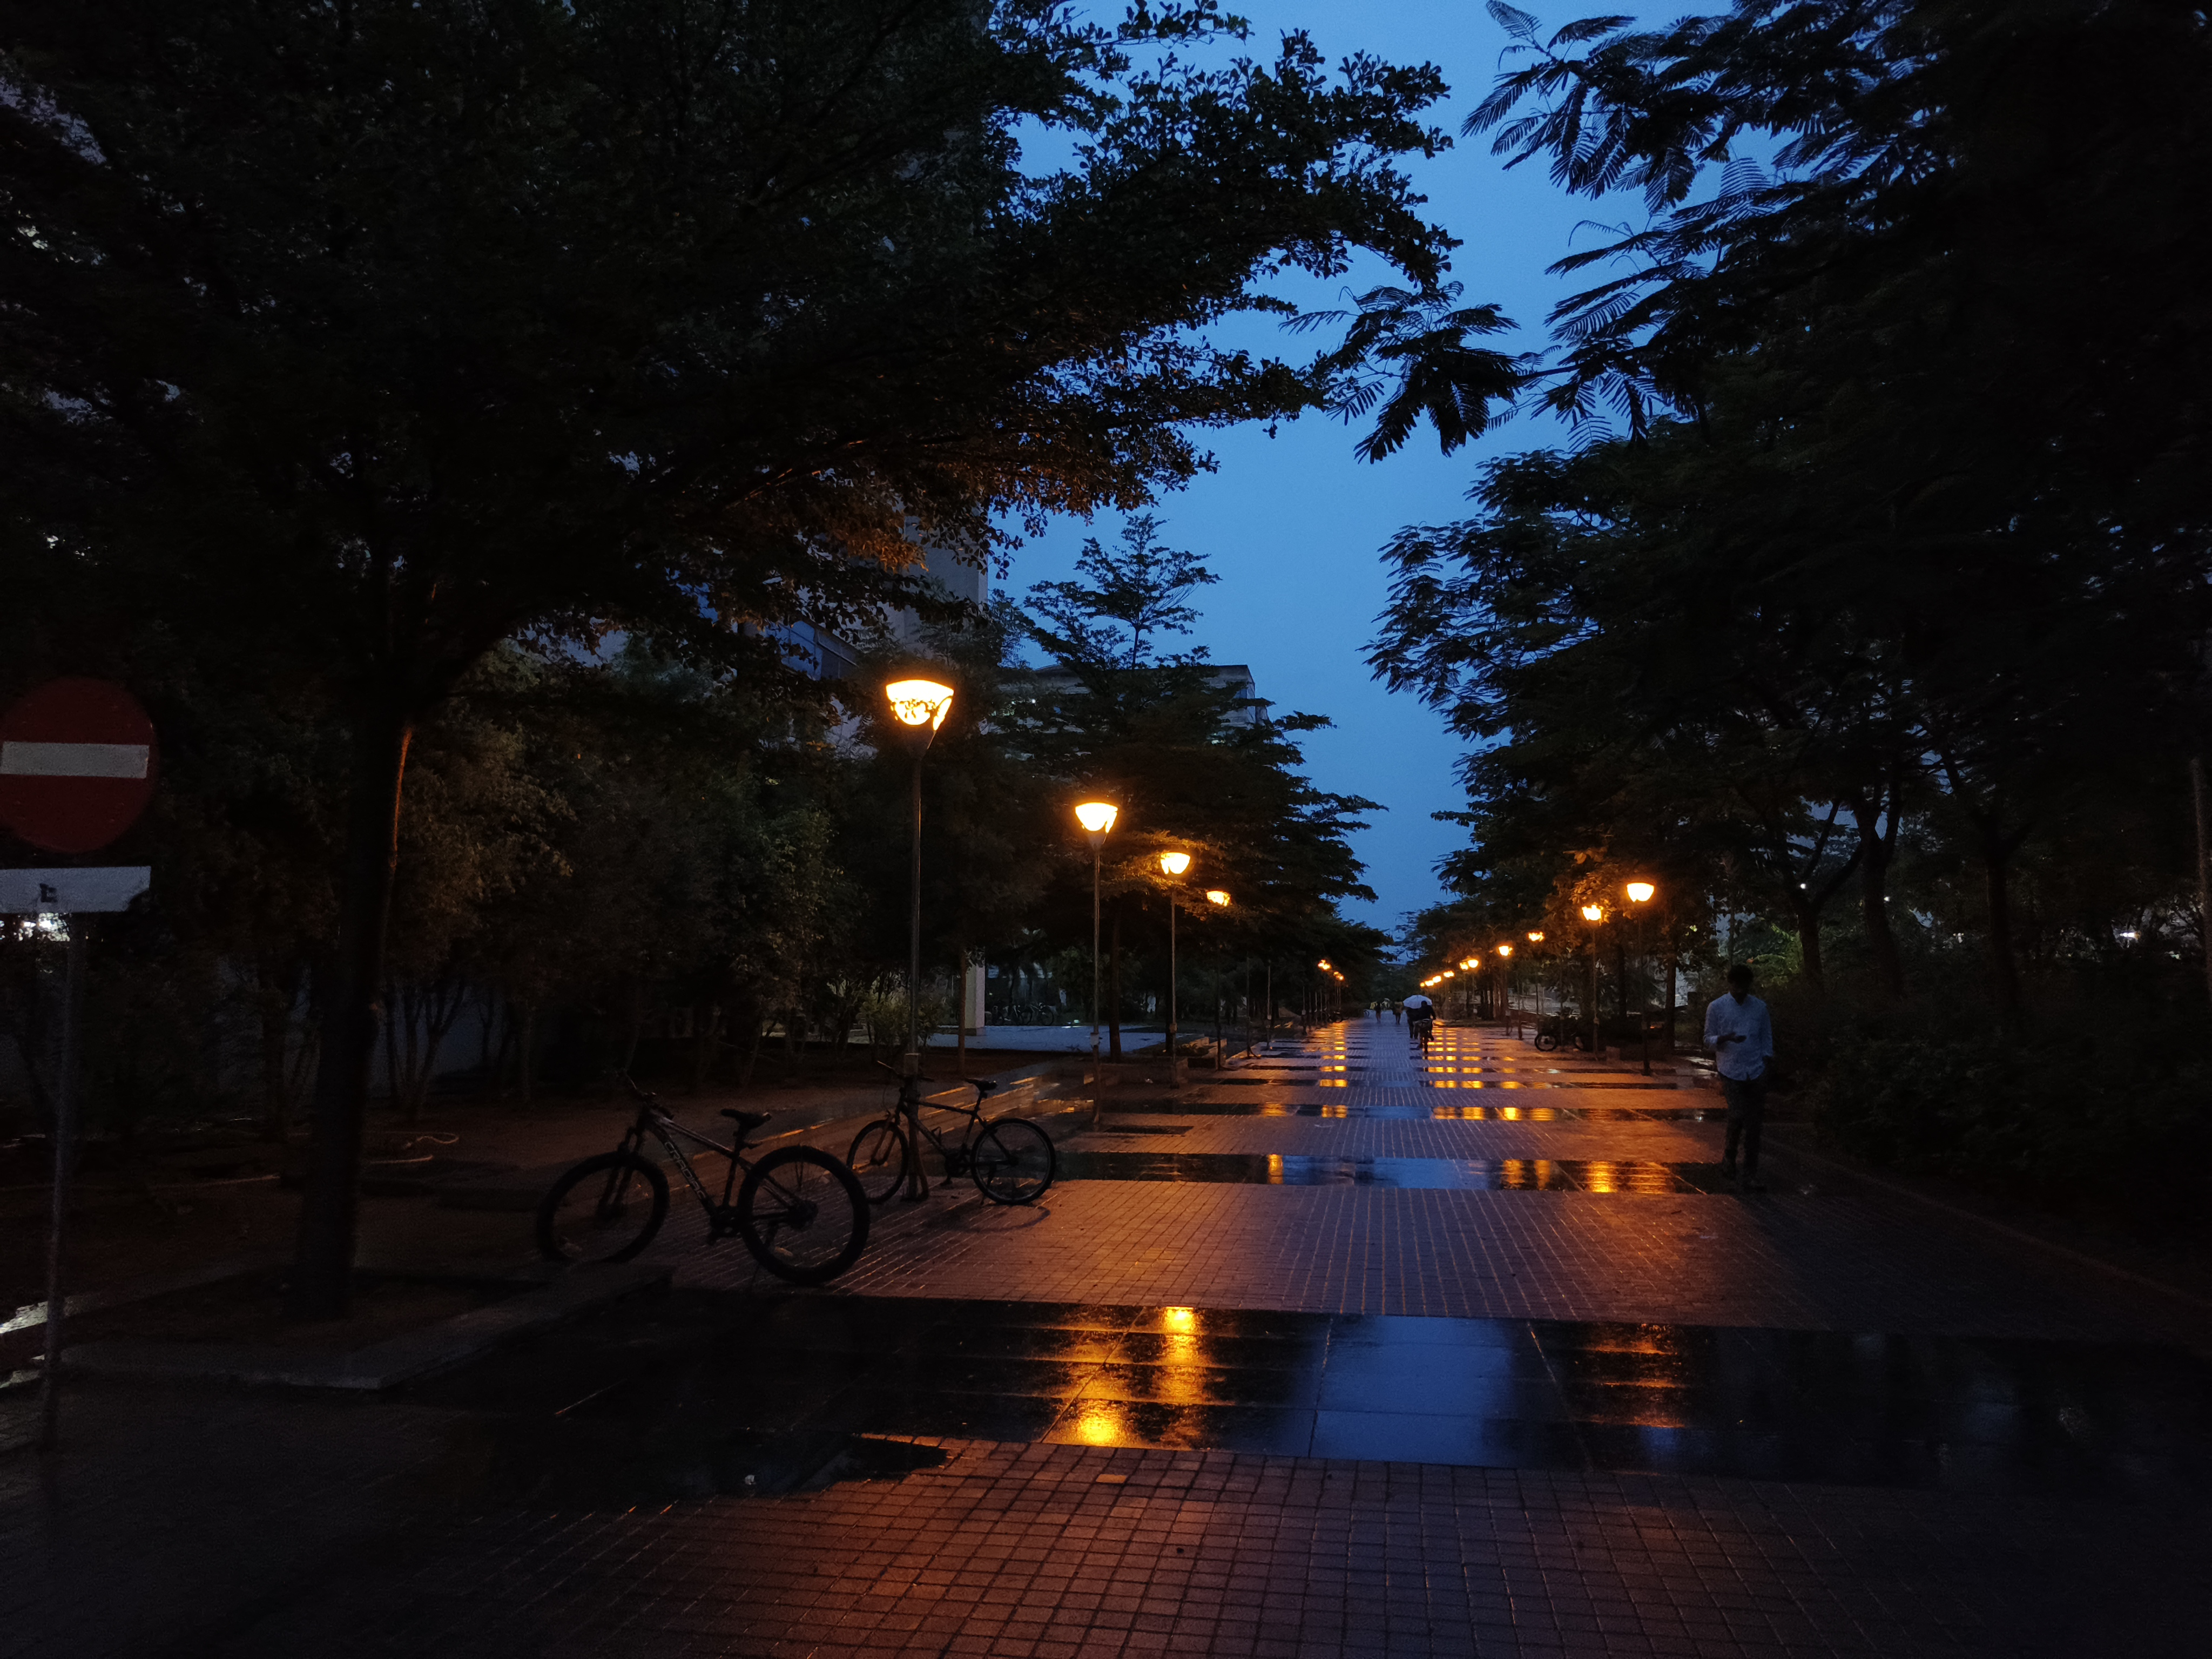
\includegraphics[width=0.5\linewidth]{figs/scenery/input.jpg}
    \caption{Input scenery image.}
    \label{fig:scenery_input}
\end{figure}

\begin{figure}[H]
    \centering
    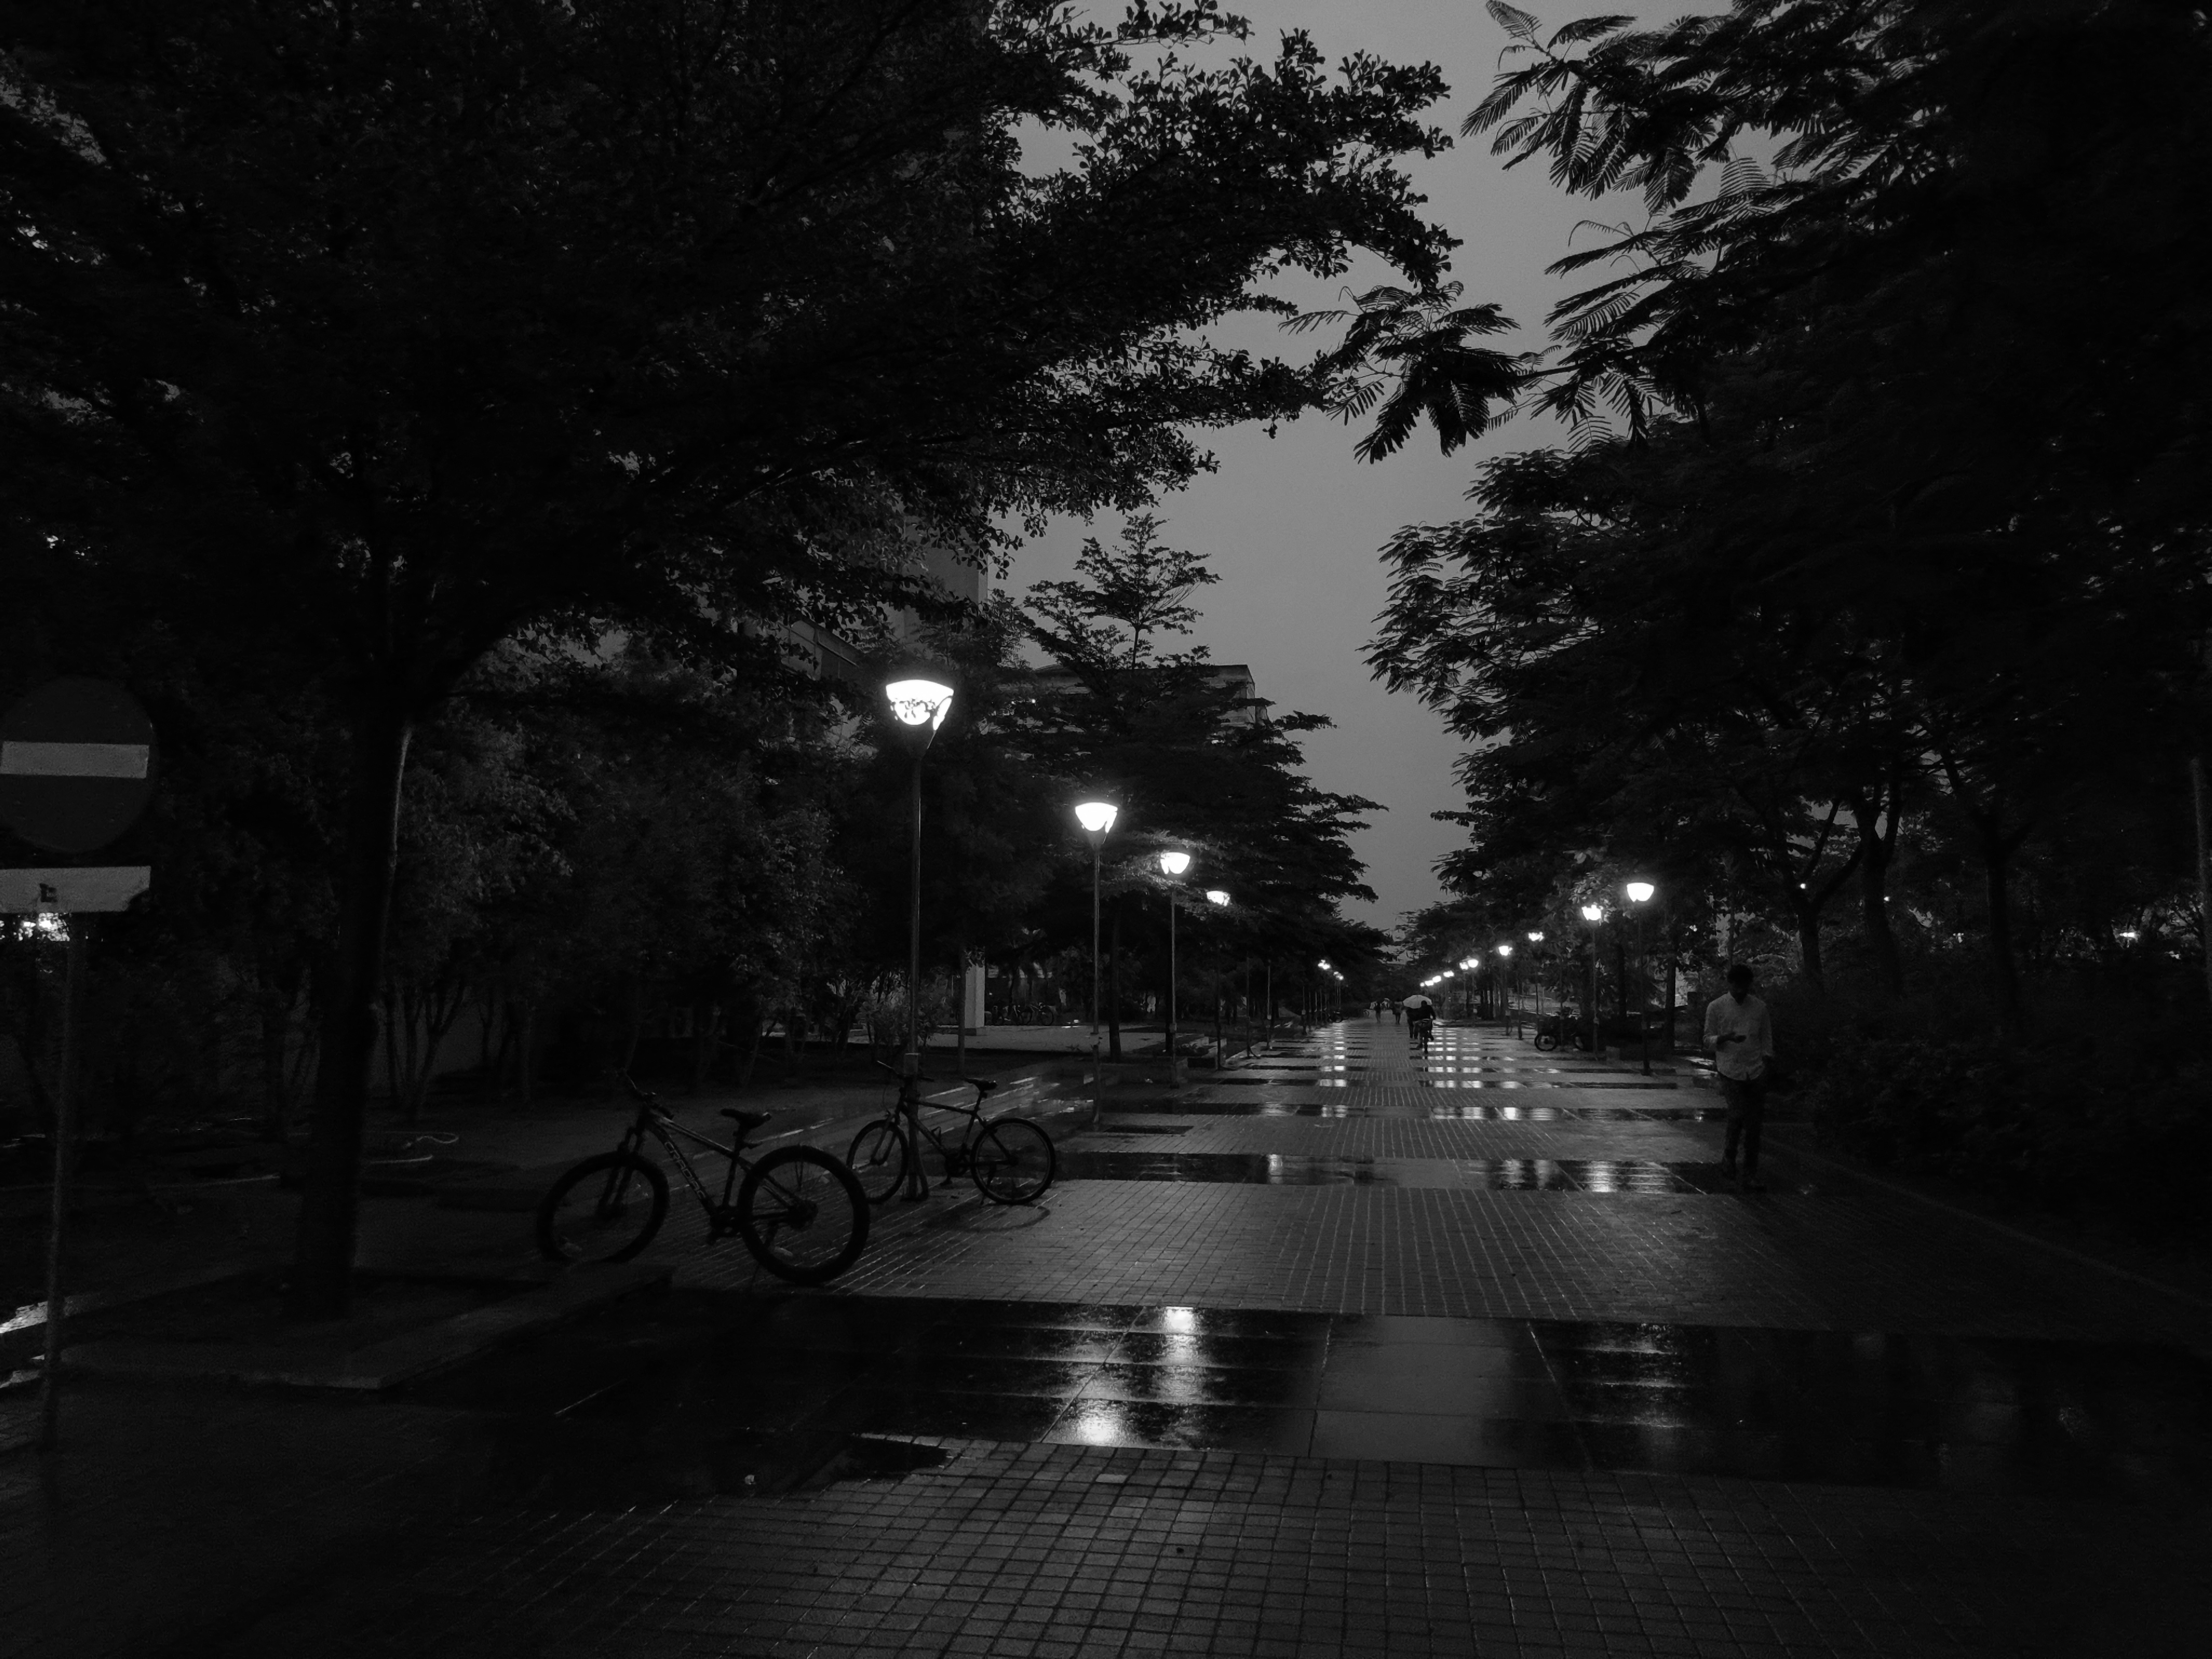
\includegraphics[width=0.5\linewidth]{figs/scenery/output_grayscale.pdf}
    \caption{Grayscale representation of the scenery image.}
    \label{fig:scenery_grayscale}
\end{figure}

\begin{figure}[H]
    \centering
    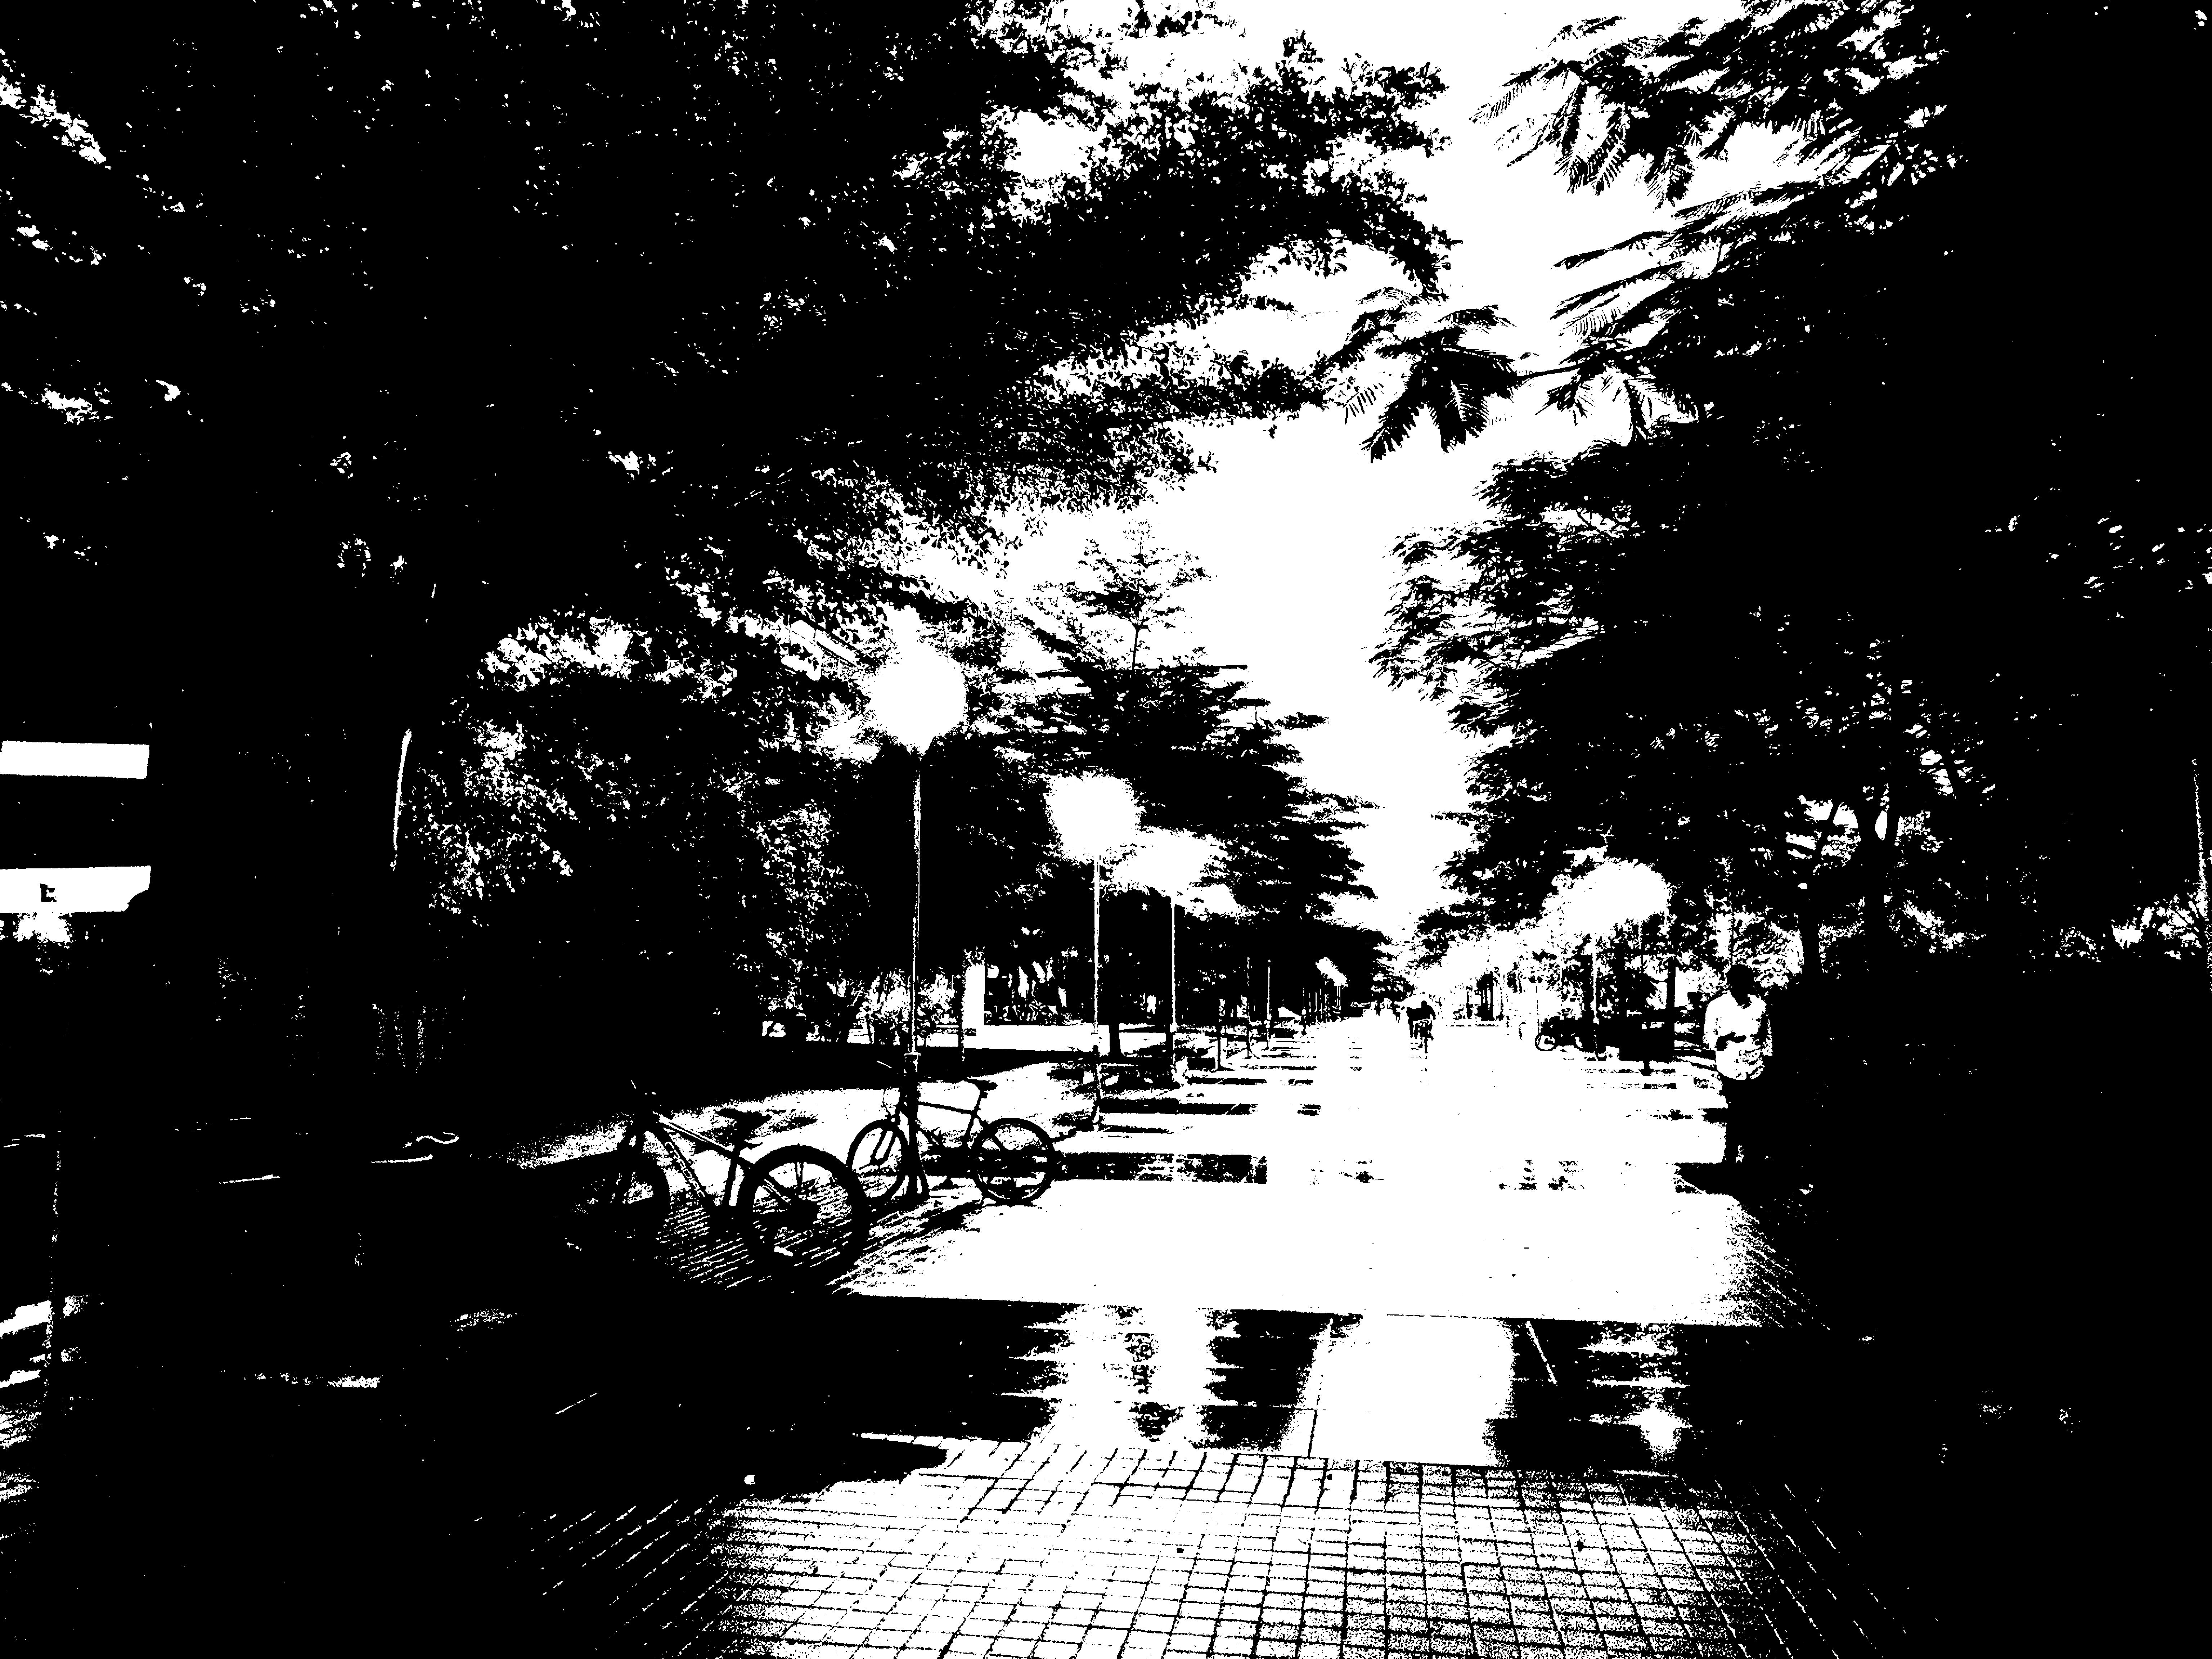
\includegraphics[width=0.5\linewidth]{figs/scenery/averaged_reference.pdf}
    \caption{Global mean adaptive thresholding of the scenery image.}
    \label{fig:scenery_adaptive}
\end{figure}

\begin{figure}[H]
    \centering
    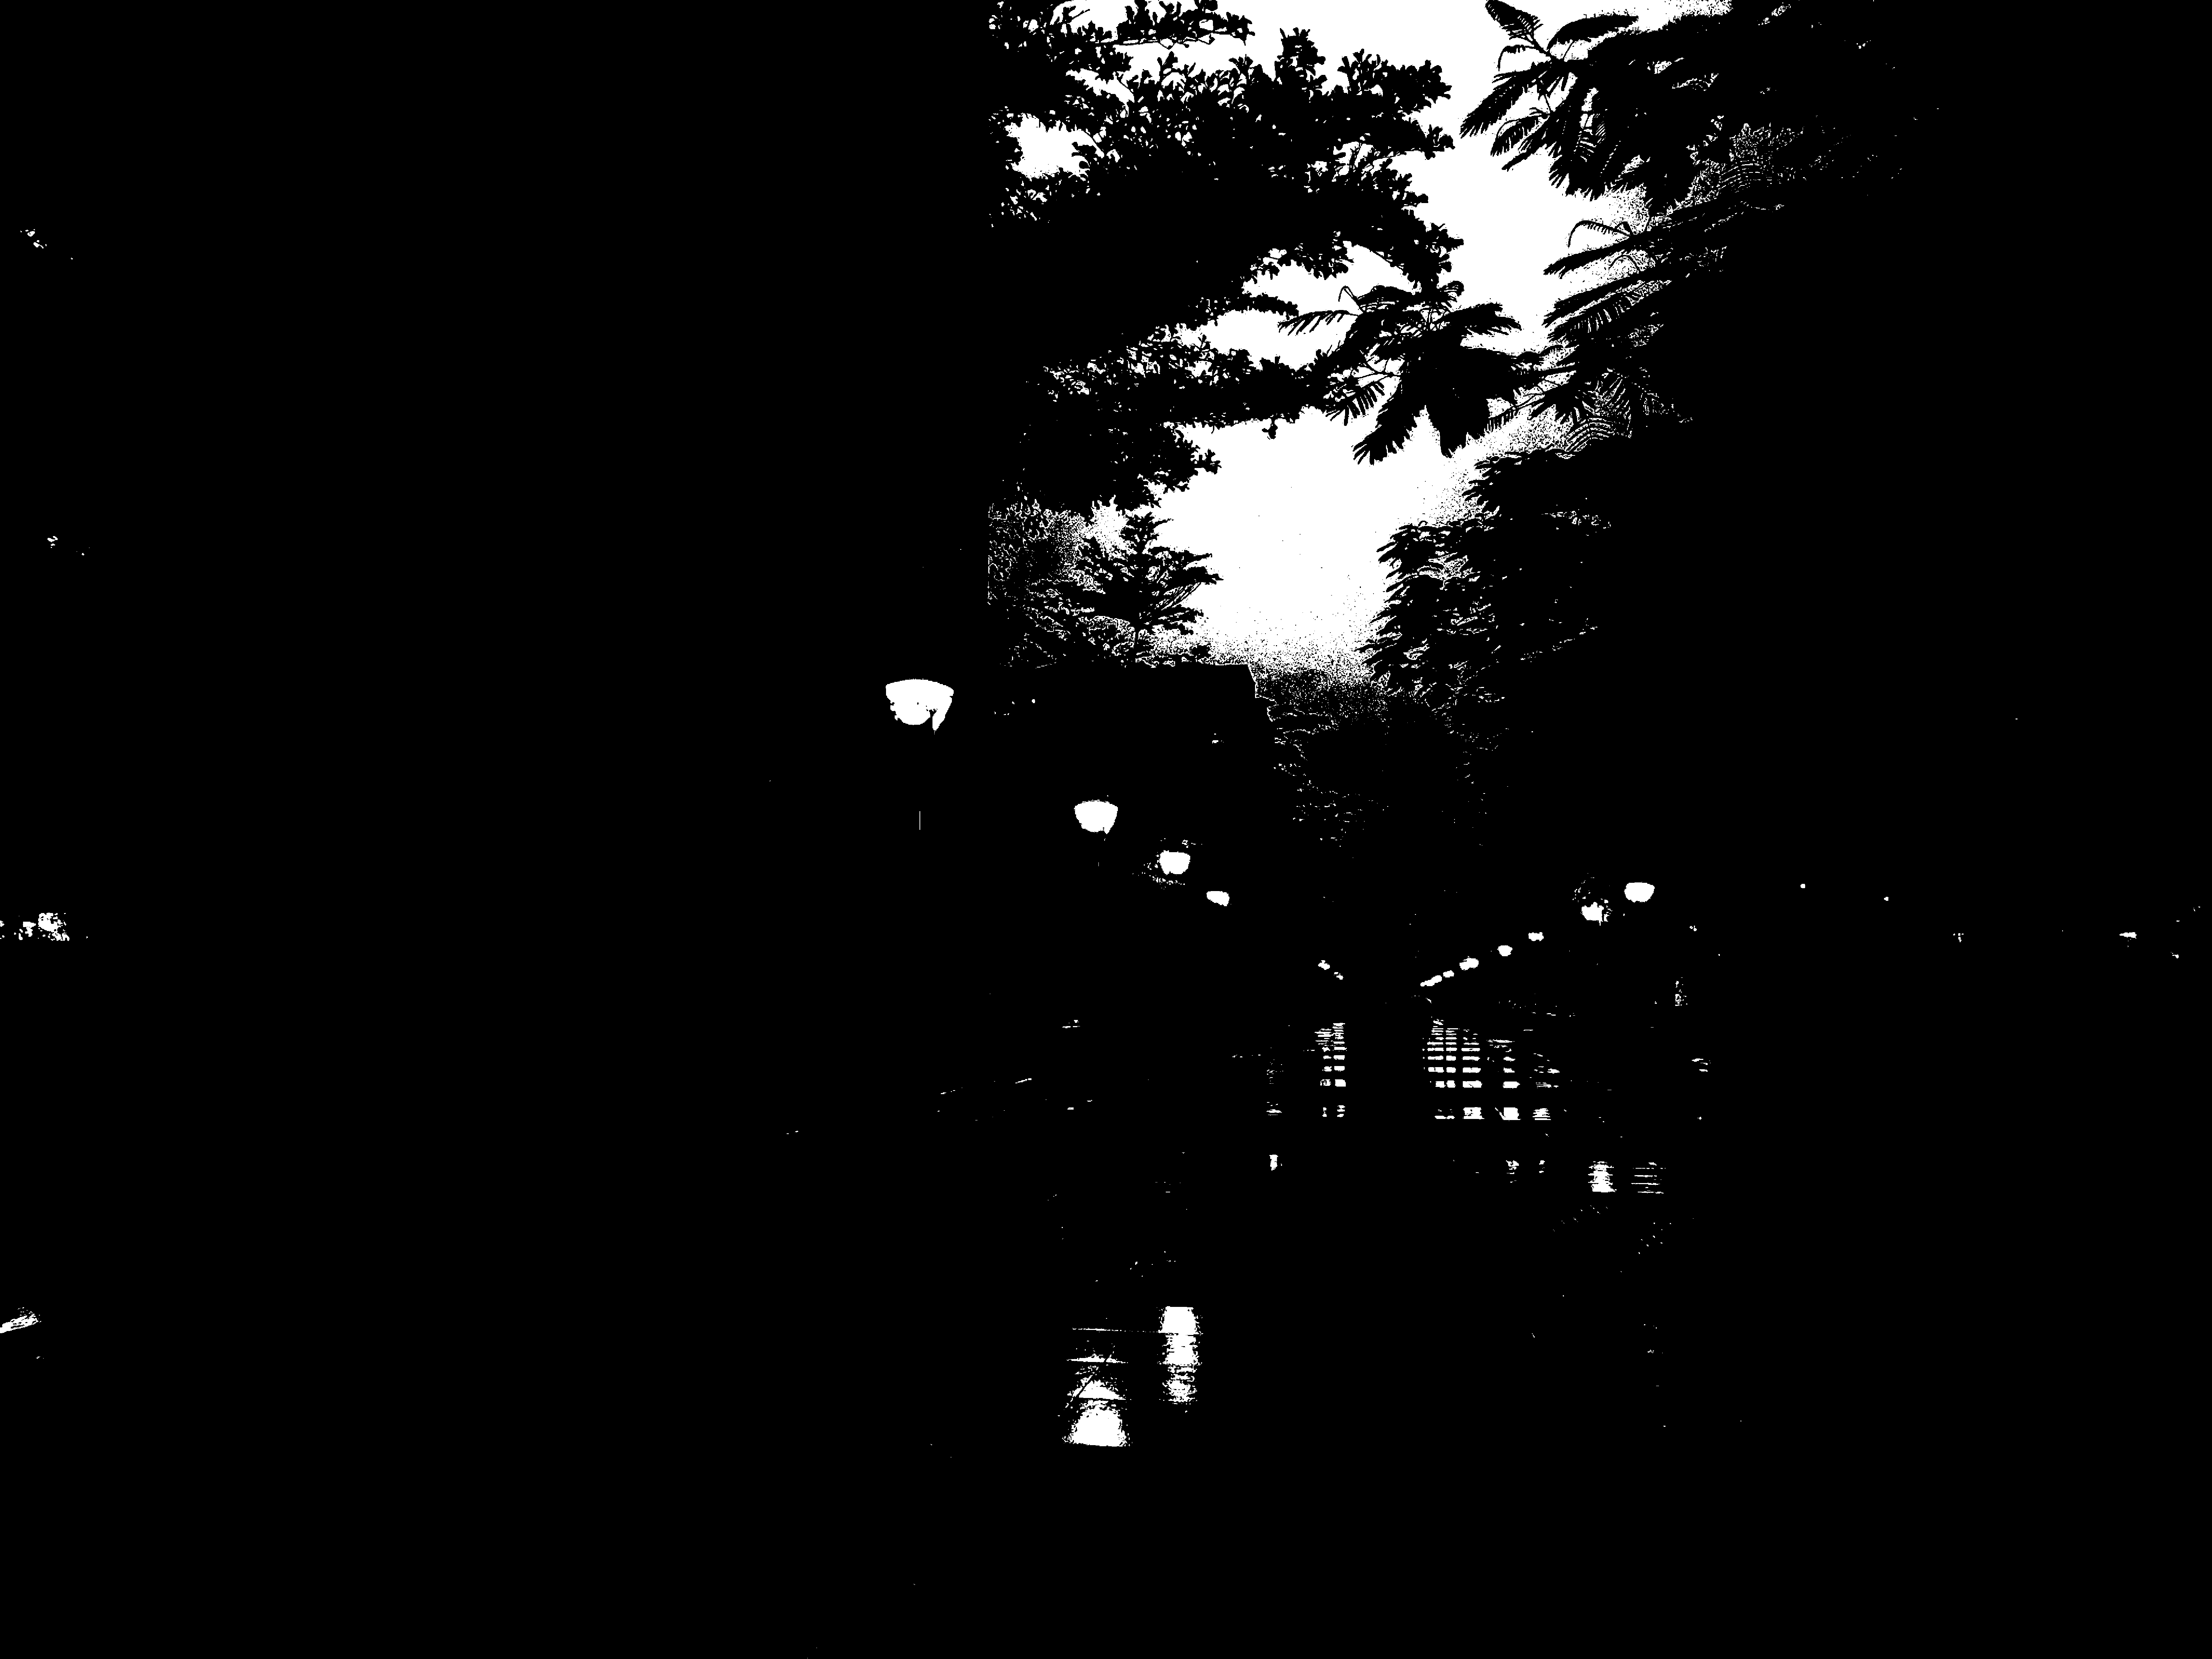
\includegraphics[width=0.5\linewidth]{figs/scenery/fixed_reference.pdf}
    \caption{Static thresholding using the fixed reference of $128$.}
    \label{fig:scenery_static}
\end{figure}

\begin{figure}[H]
    \centering
    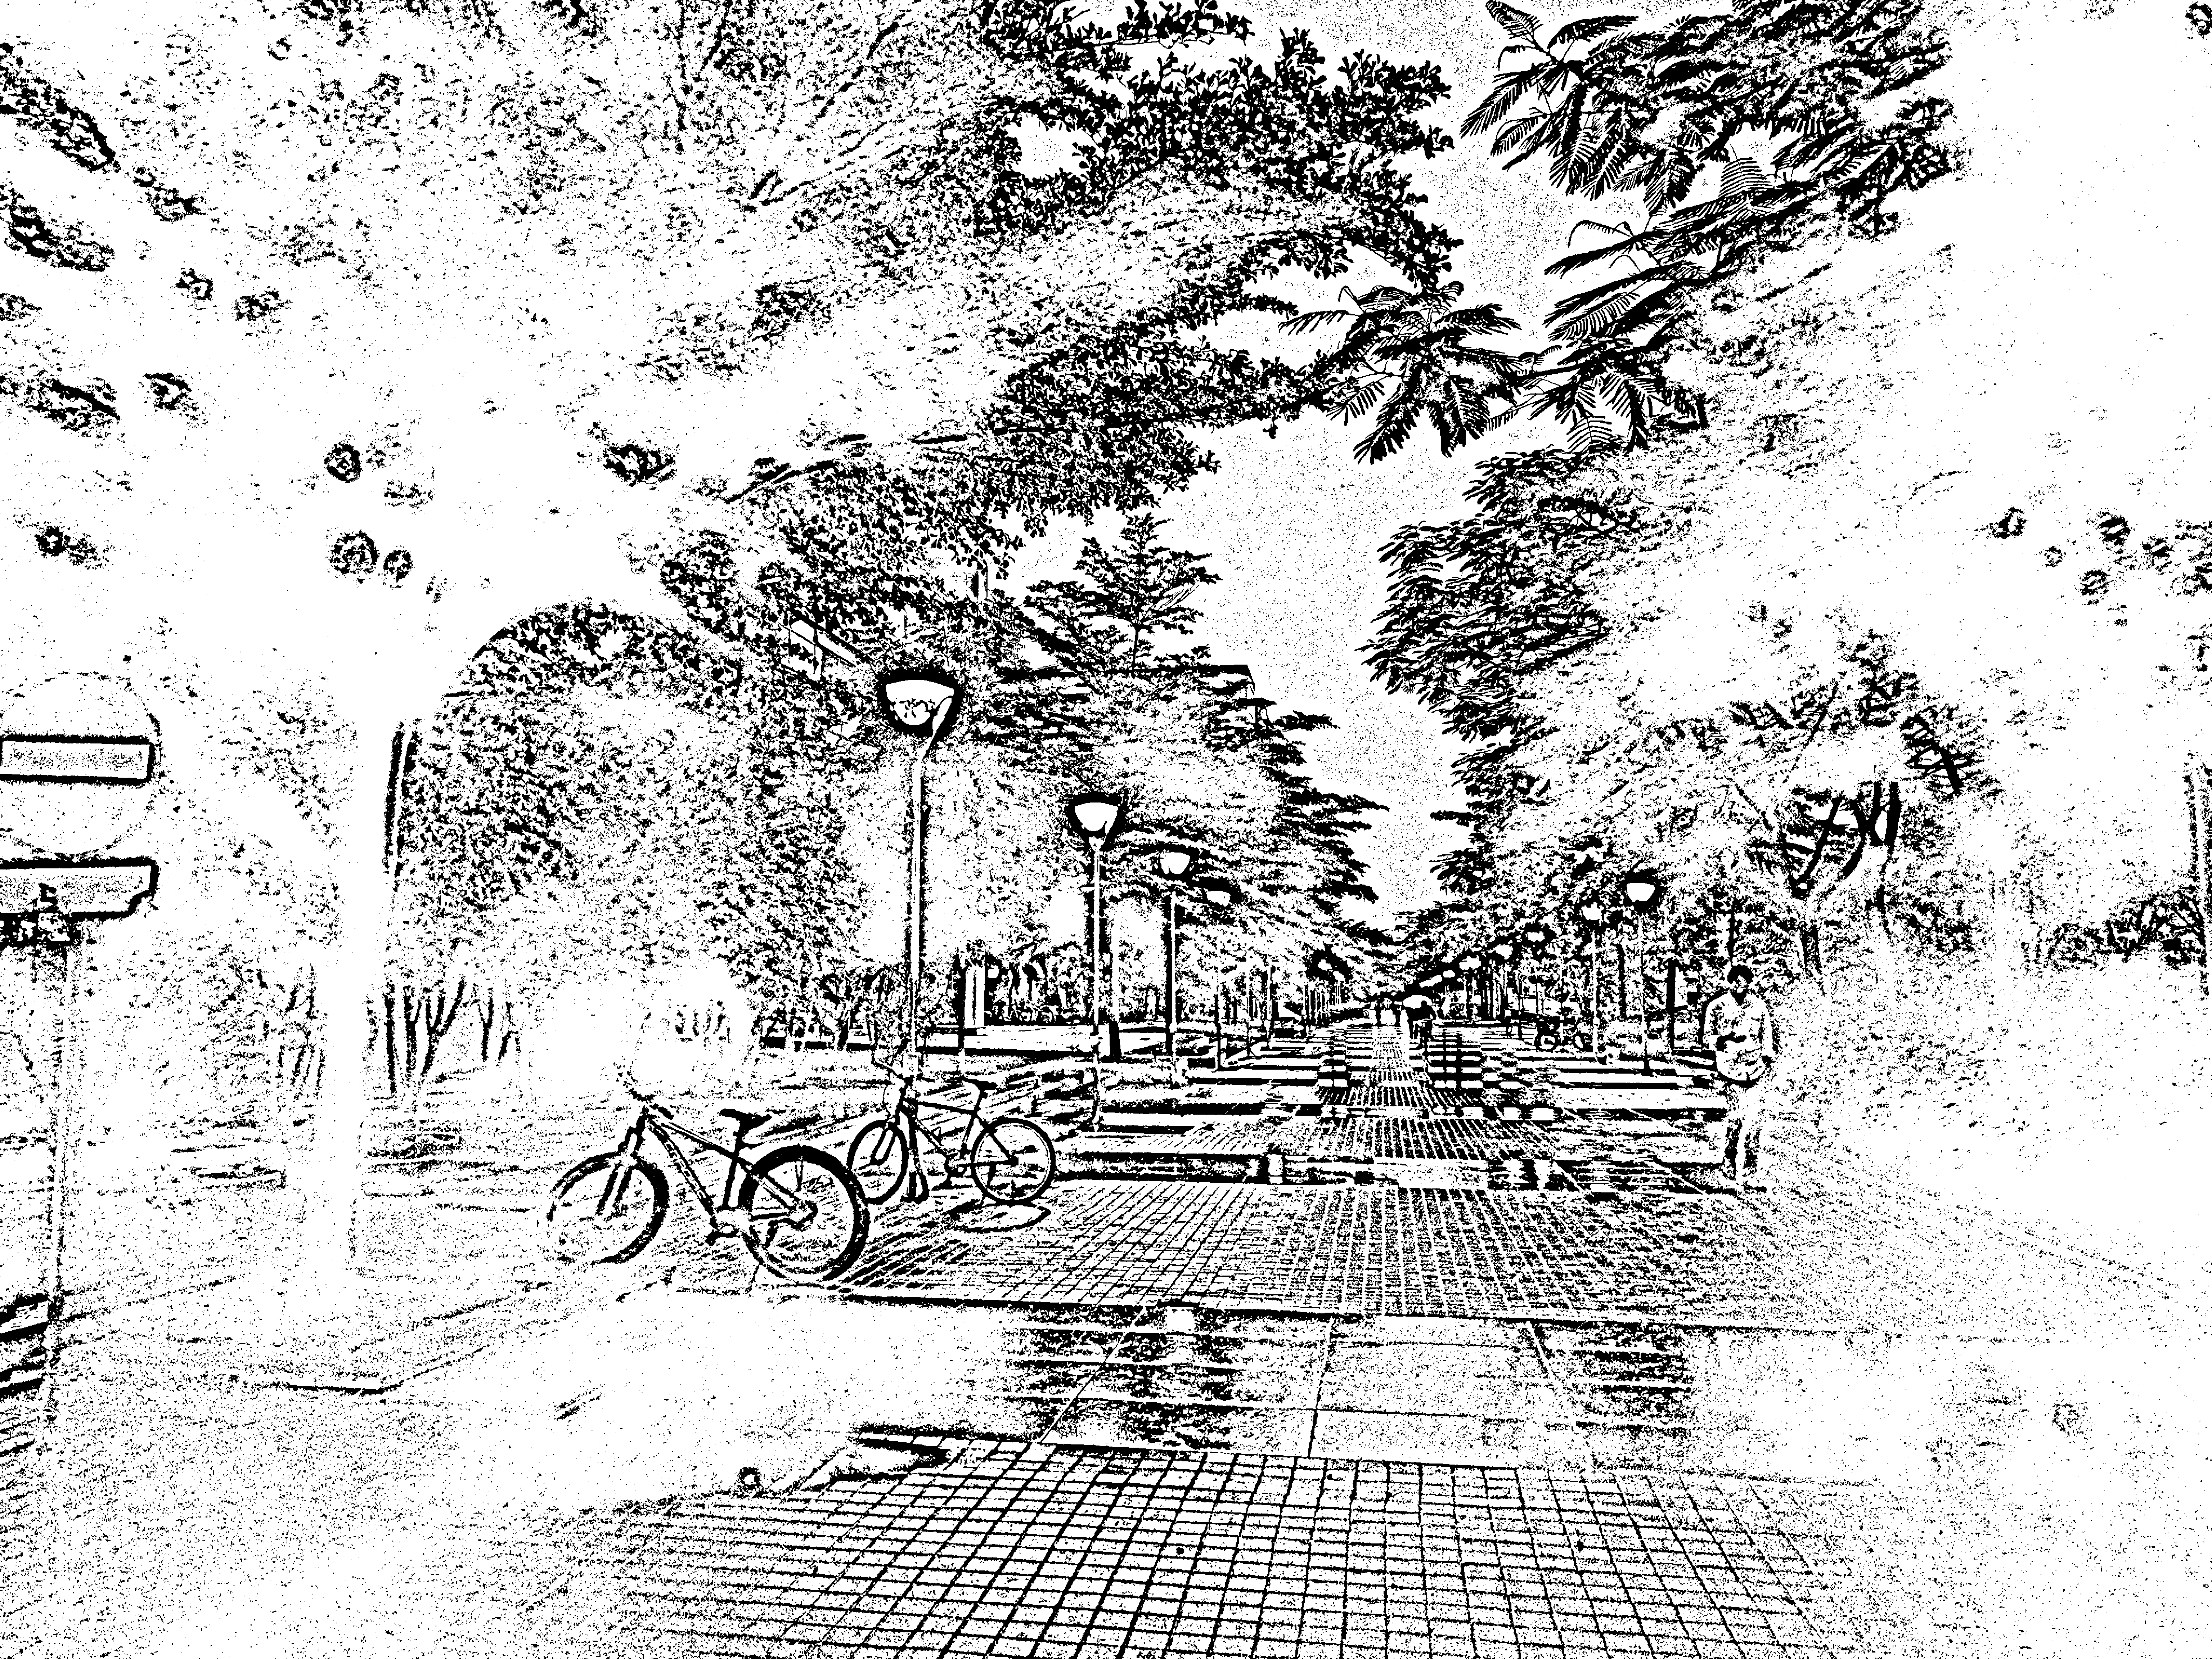
\includegraphics[width=0.5\linewidth]{figs/scenery/gaussian_localized_reference.pdf}
    \caption{Gaussian localized reference with $\sigma=10$ and $C=3$.}
    \label{fig:scenery_gaussian_localized}
\end{figure}

\begin{figure}[H]
    \centering
    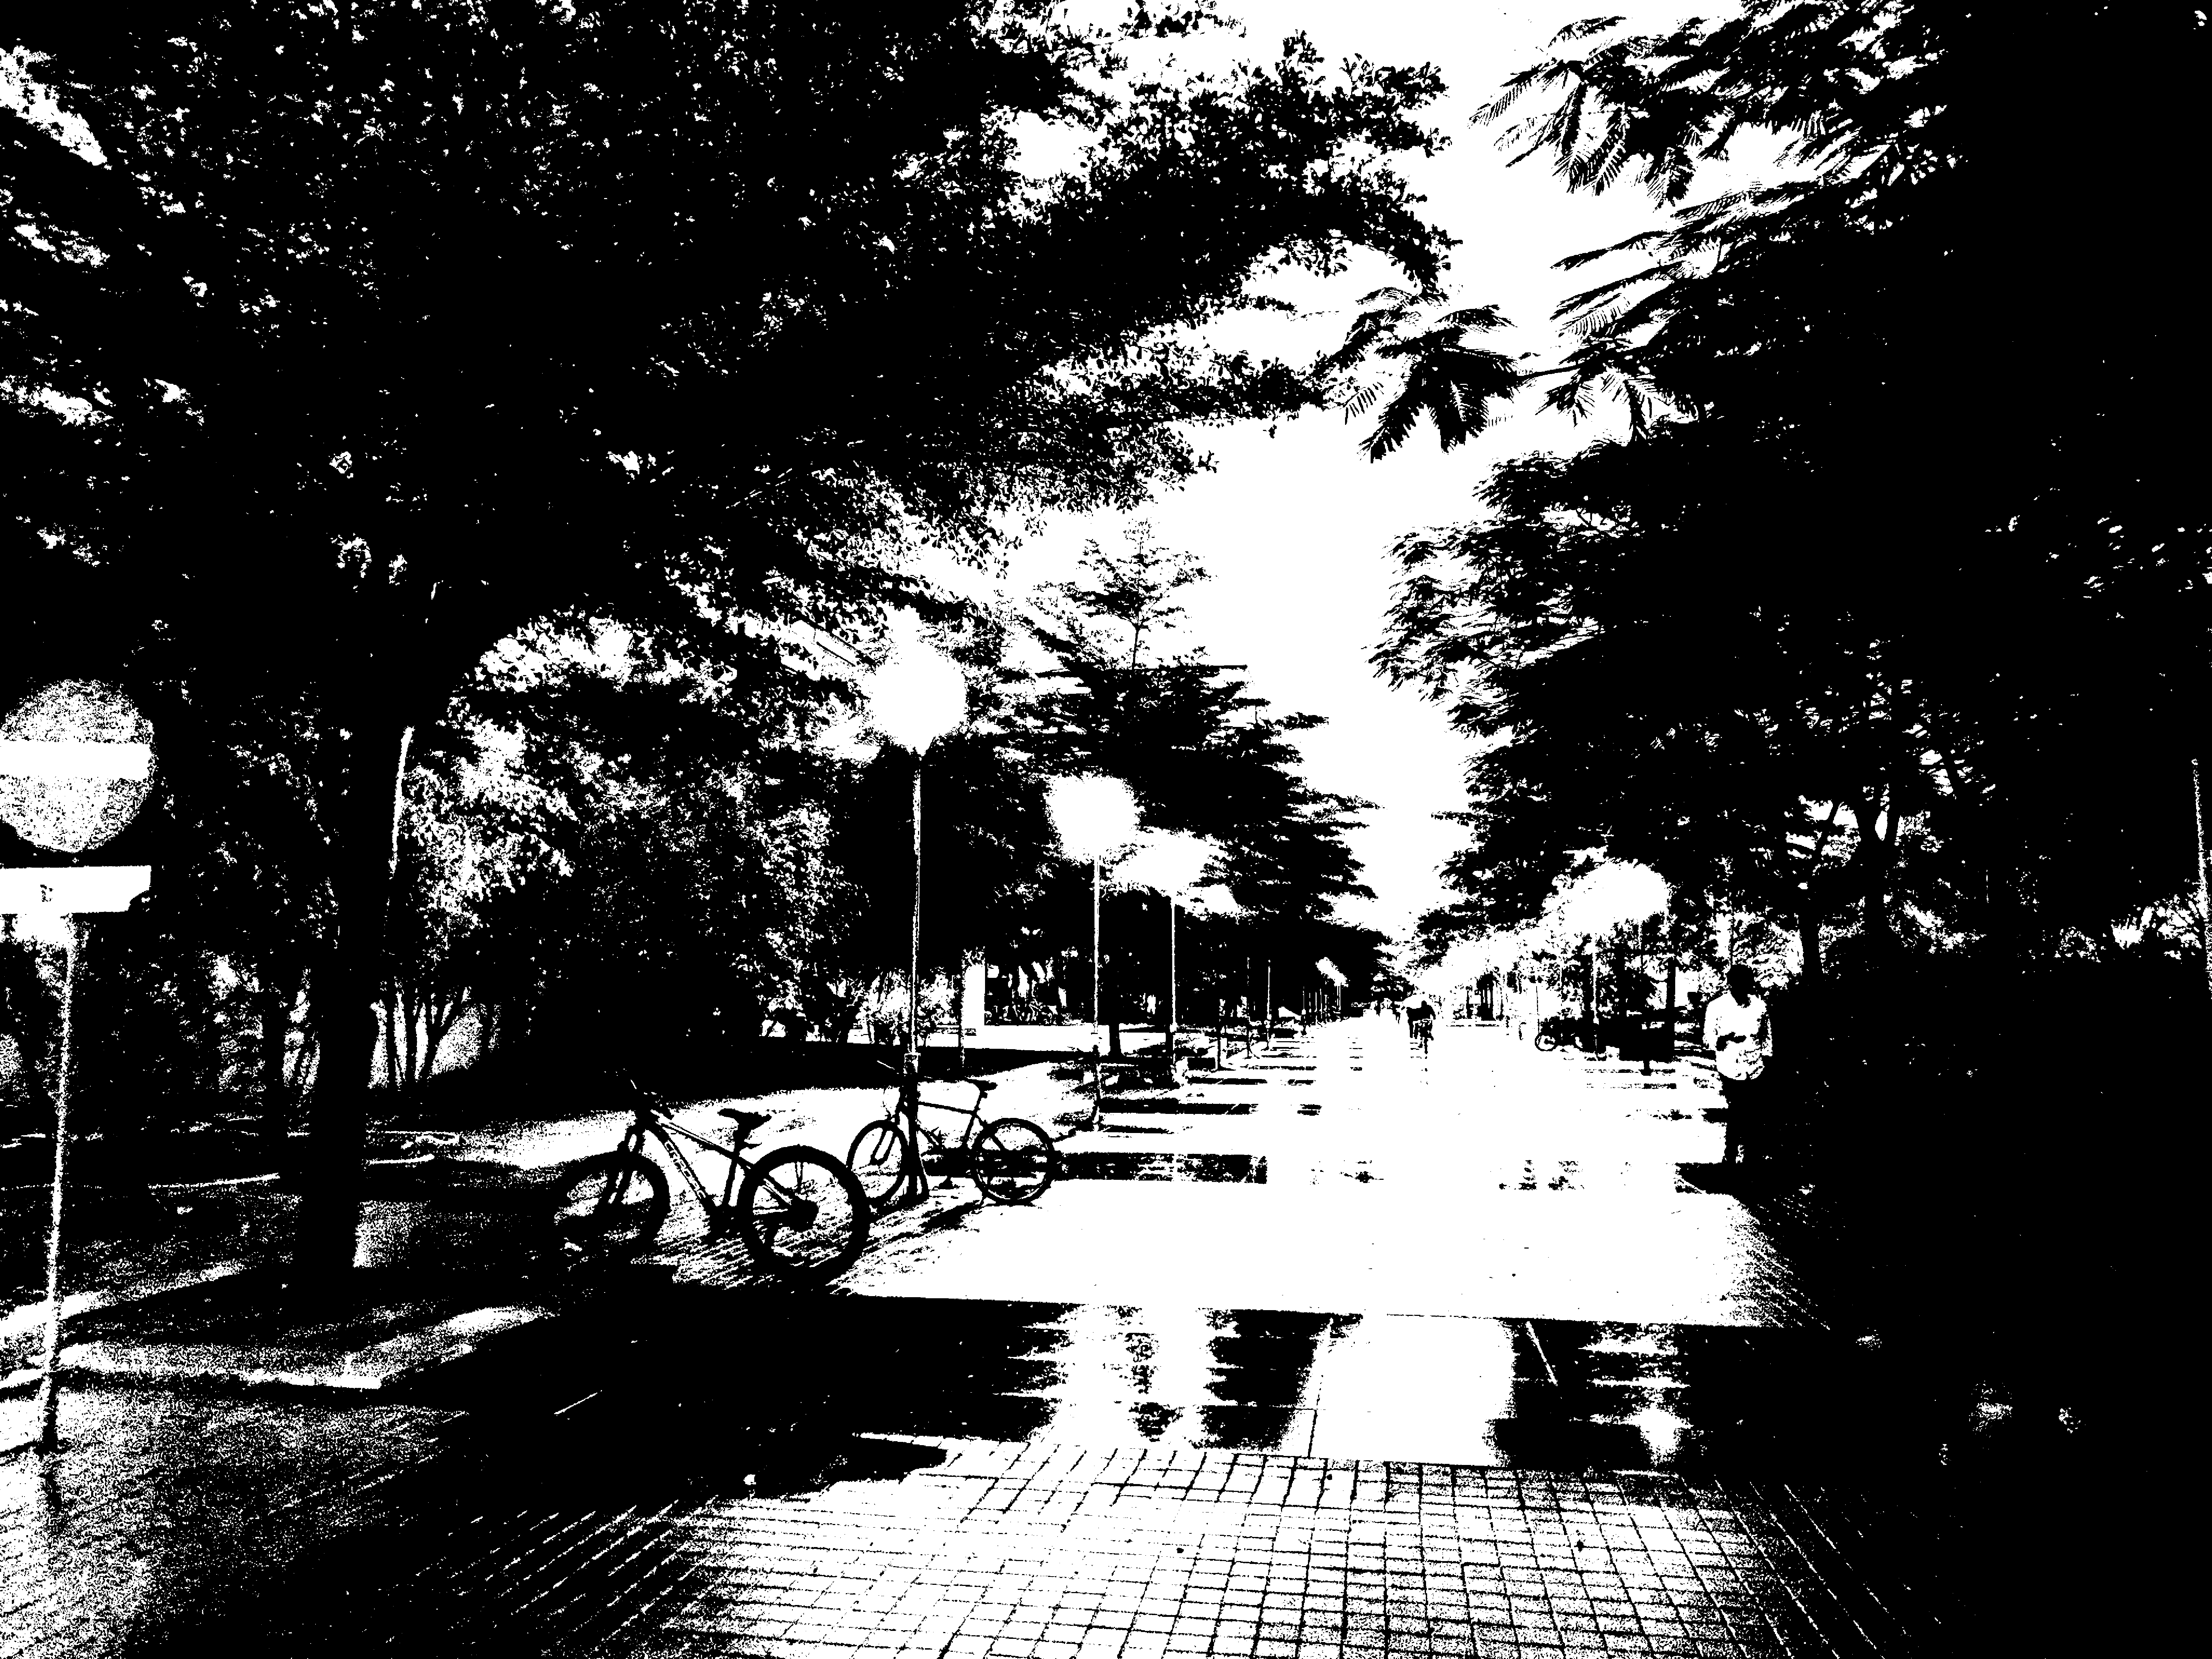
\includegraphics[width=0.5\linewidth]{figs/scenery/gaussian_wide_reference.pdf}
    \caption{Gaussian wide reference with $\sigma=1200$ and $C=3$.}
    \label{fig:scenery_gaussian_wide}
\end{figure}
\vspace*{\baselineskip}
\subsection{Testing Case 2: Jersey}

The second test case uses a jersey image. The same sequence is retained
to make the behaviour of the reference methods directly comparable.

\begin{figure}[H]
    \centering
    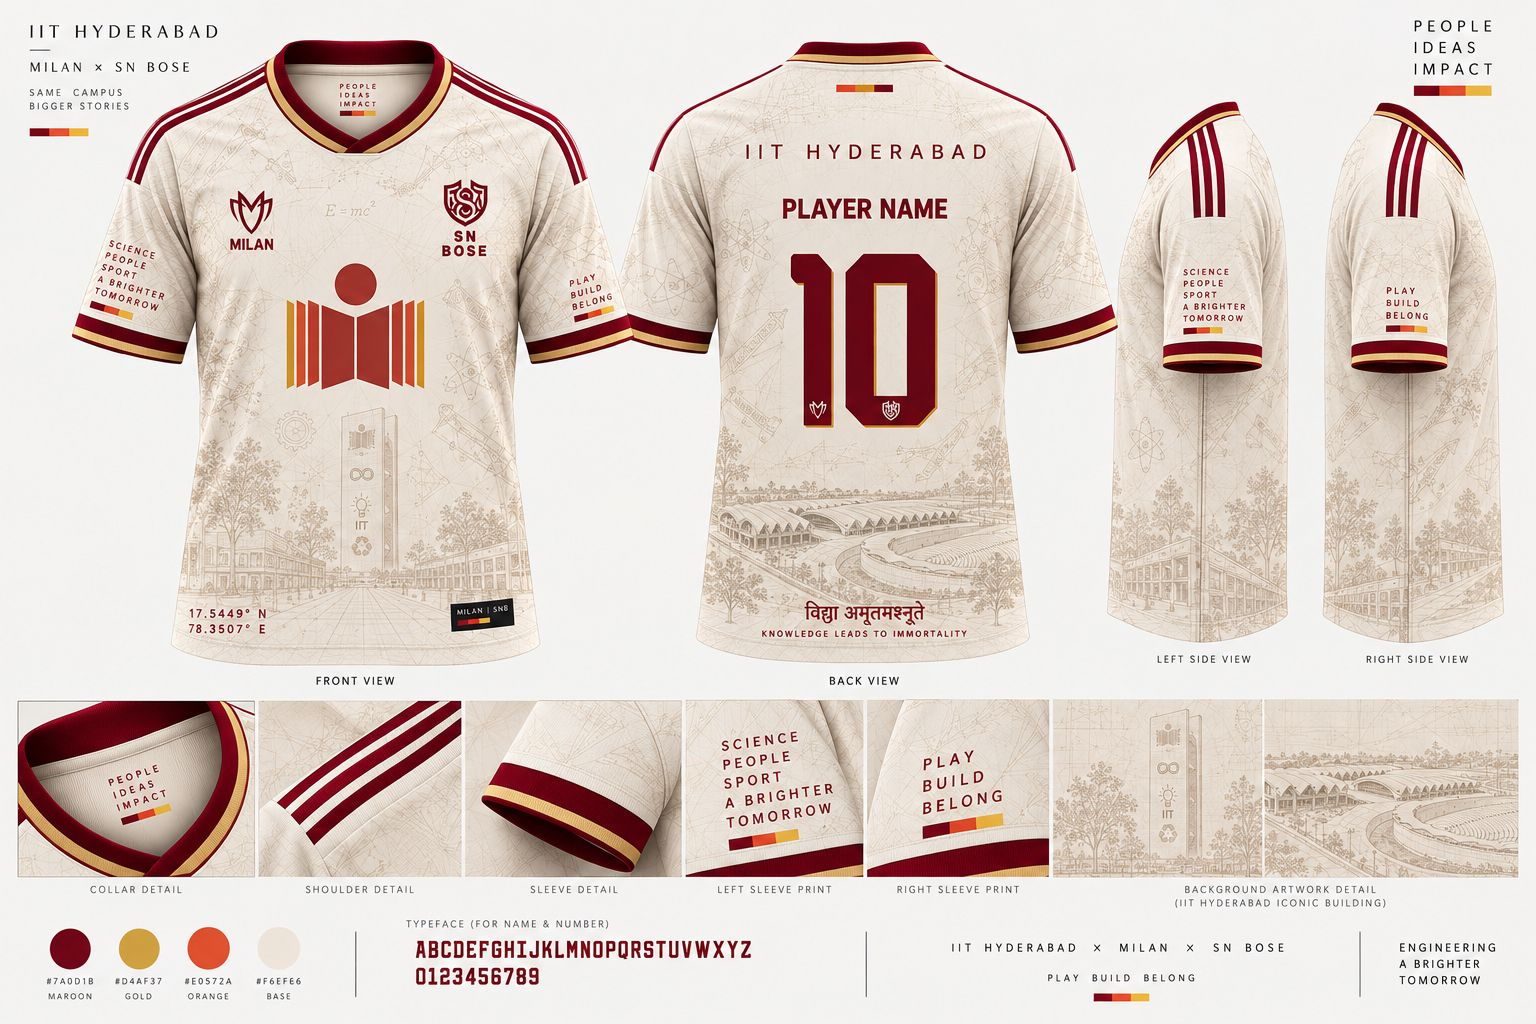
\includegraphics[width=0.5\linewidth]{figs/jersey/input.jpg}
    \caption{Input jersey image.}
    \label{fig:jersey_input}
\end{figure}

\begin{figure}[H]
    \centering
    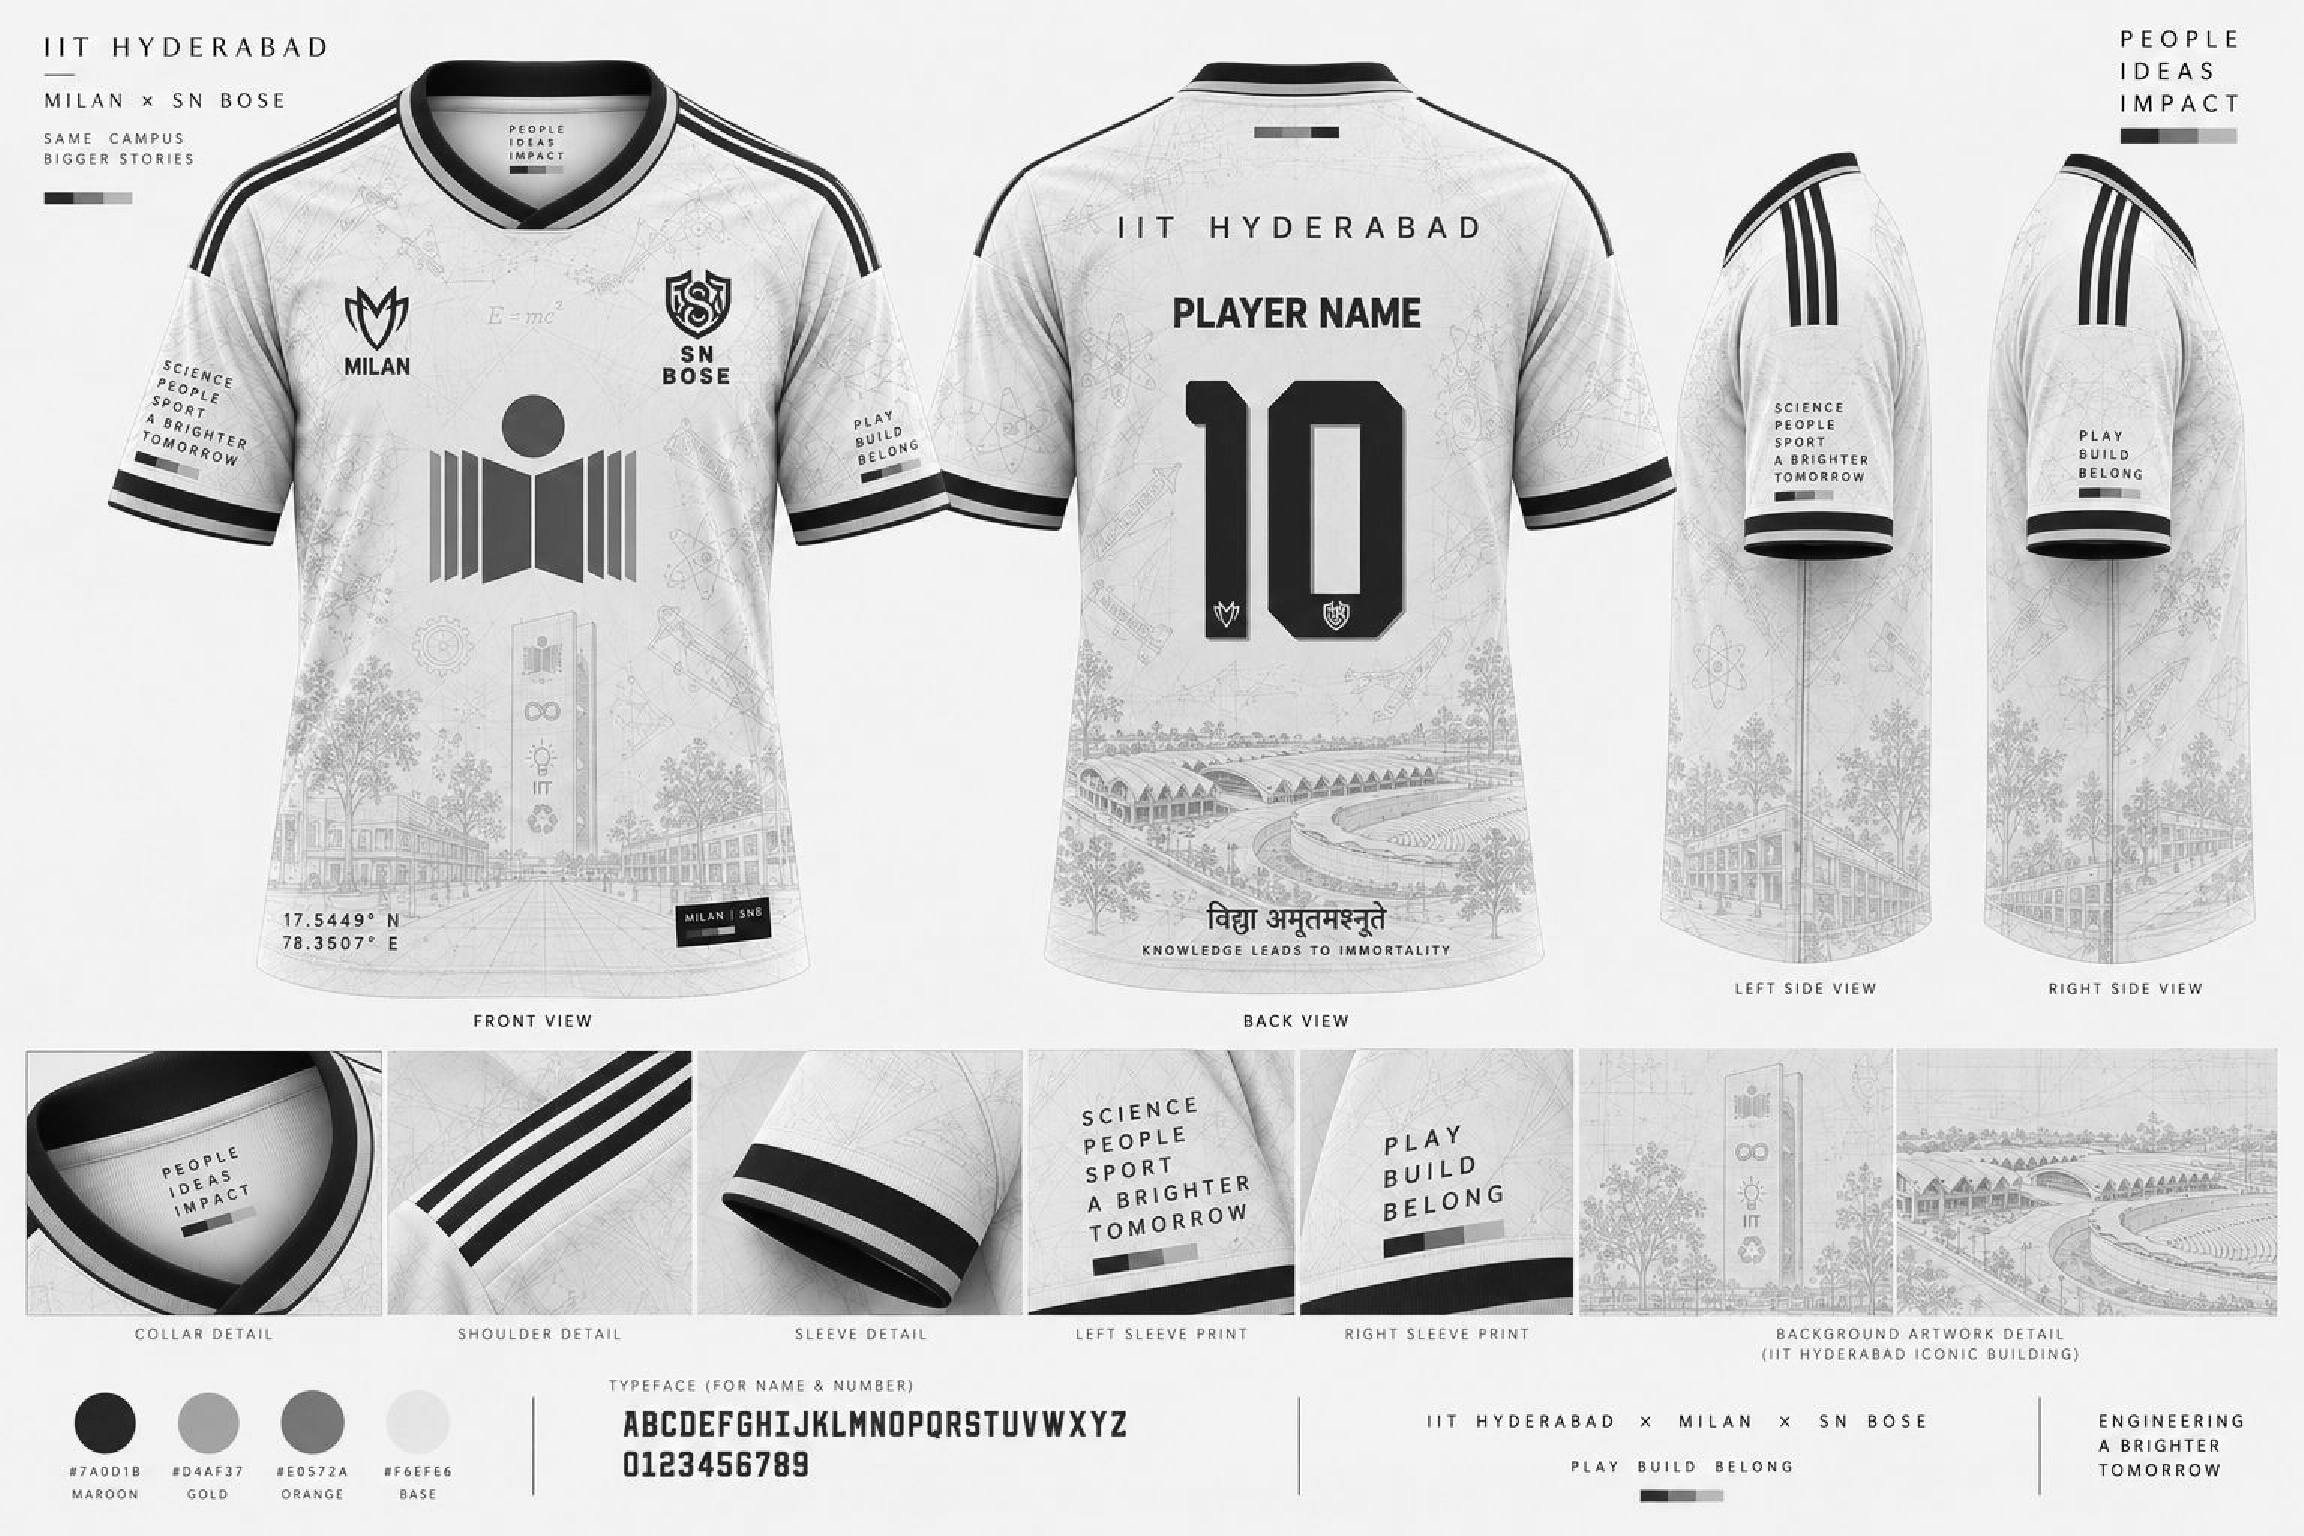
\includegraphics[width=0.5\linewidth]{figs/jersey/output_grayscale.pdf}
    \caption{Grayscale representation of the jersey image.}
    \label{fig:jersey_grayscale}
\end{figure}

\begin{figure}[H]
    \centering
    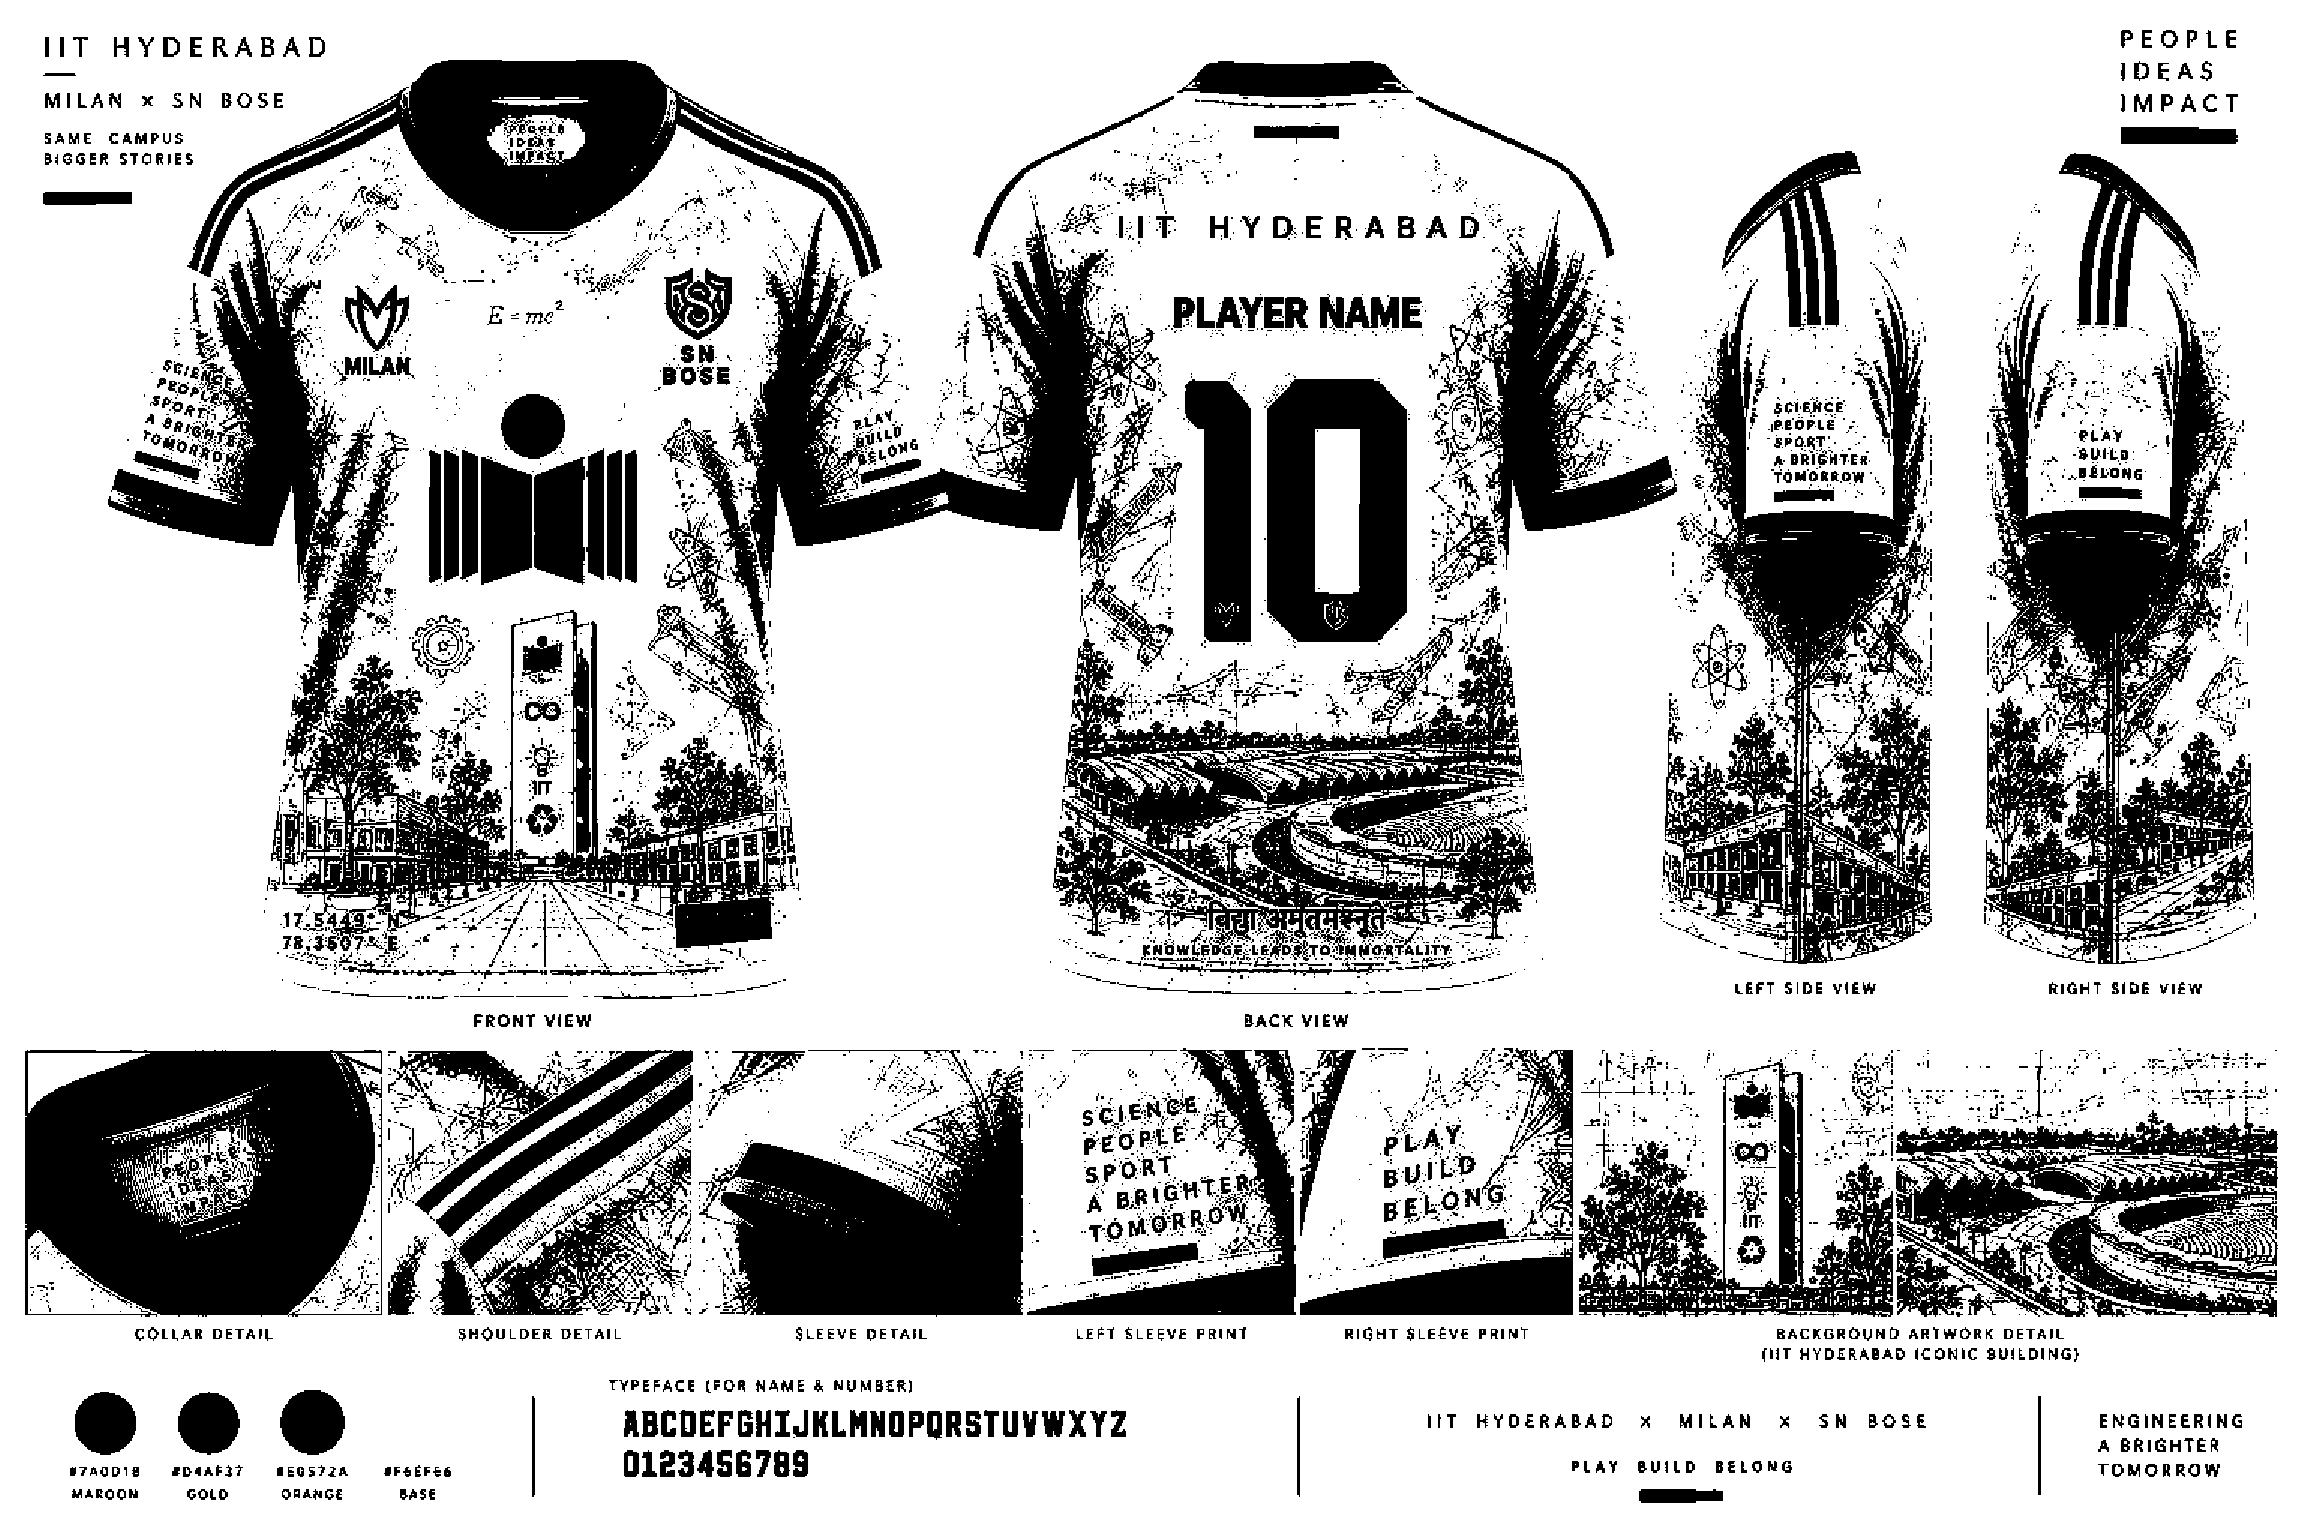
\includegraphics[width=0.5\linewidth]{figs/jersey/averaged_reference.pdf}
    \caption{Global mean adaptive thresholding of the jersey image.}
    \label{fig:jersey_adaptive}
\end{figure}

\begin{figure}[H]
    \centering
    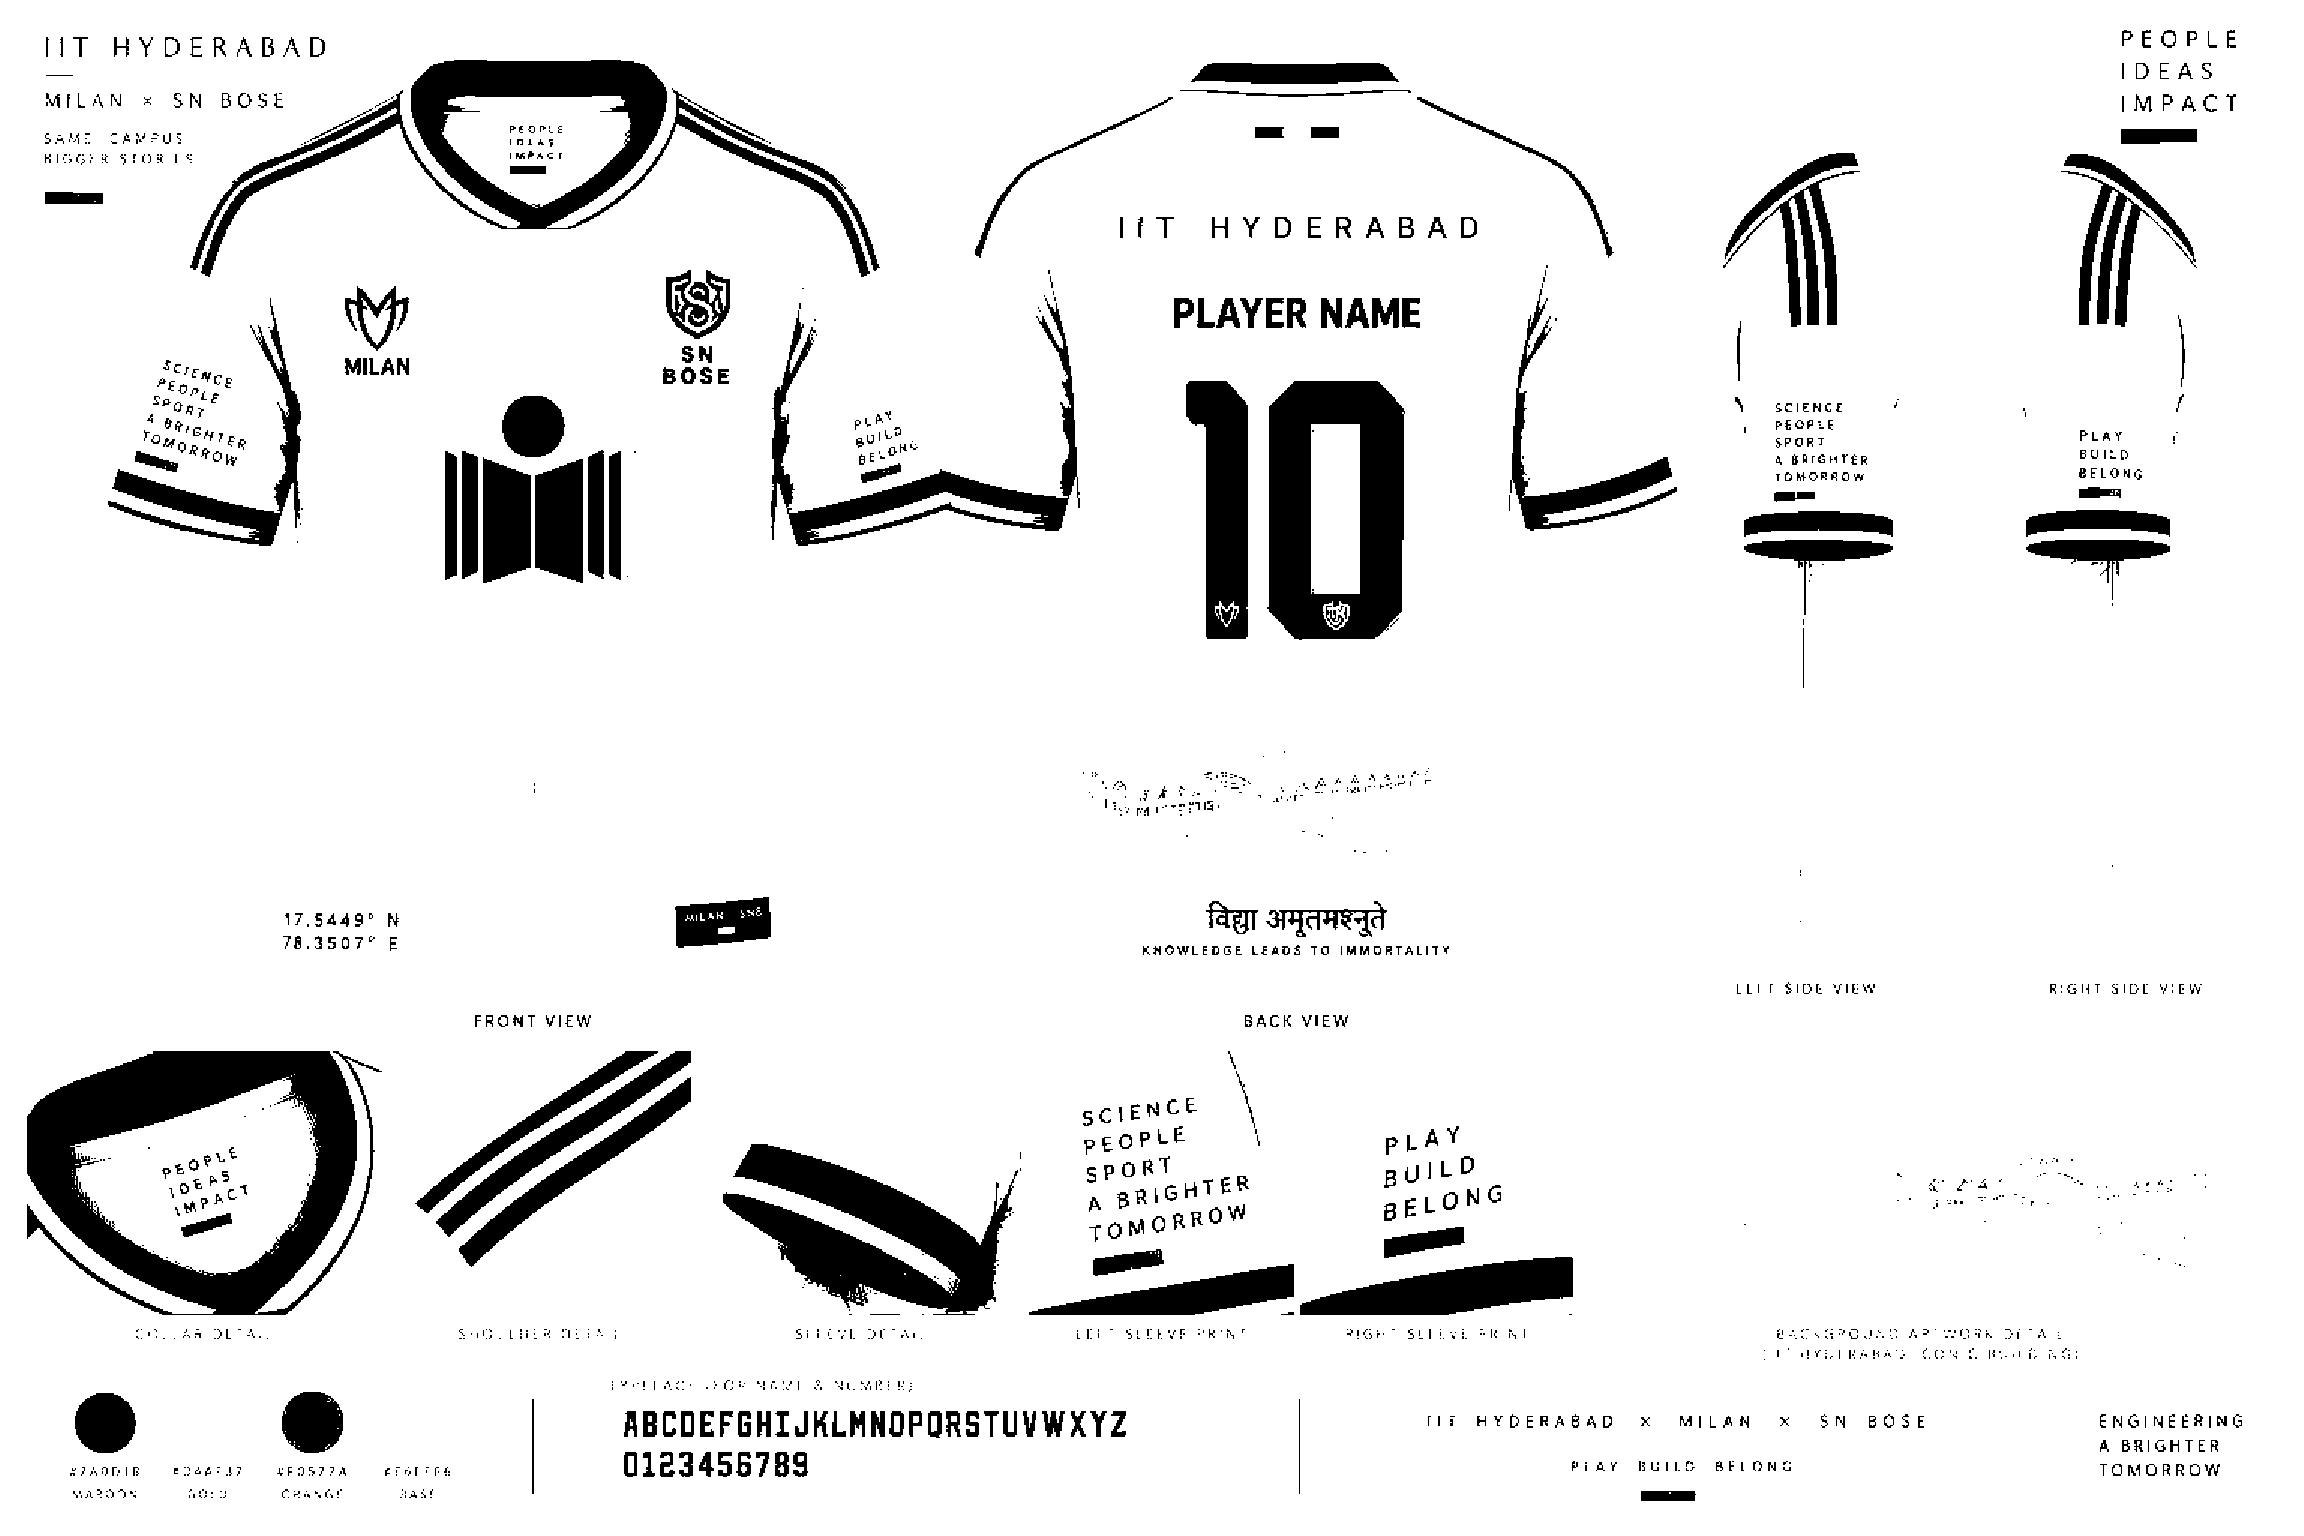
\includegraphics[width=0.5\linewidth]{figs/jersey/fixed_reference.pdf}
    \caption{Static thresholding using the fixed reference of $128$.}
    \label{fig:jersey_static}
\end{figure}

\begin{figure}[H]
    \centering
    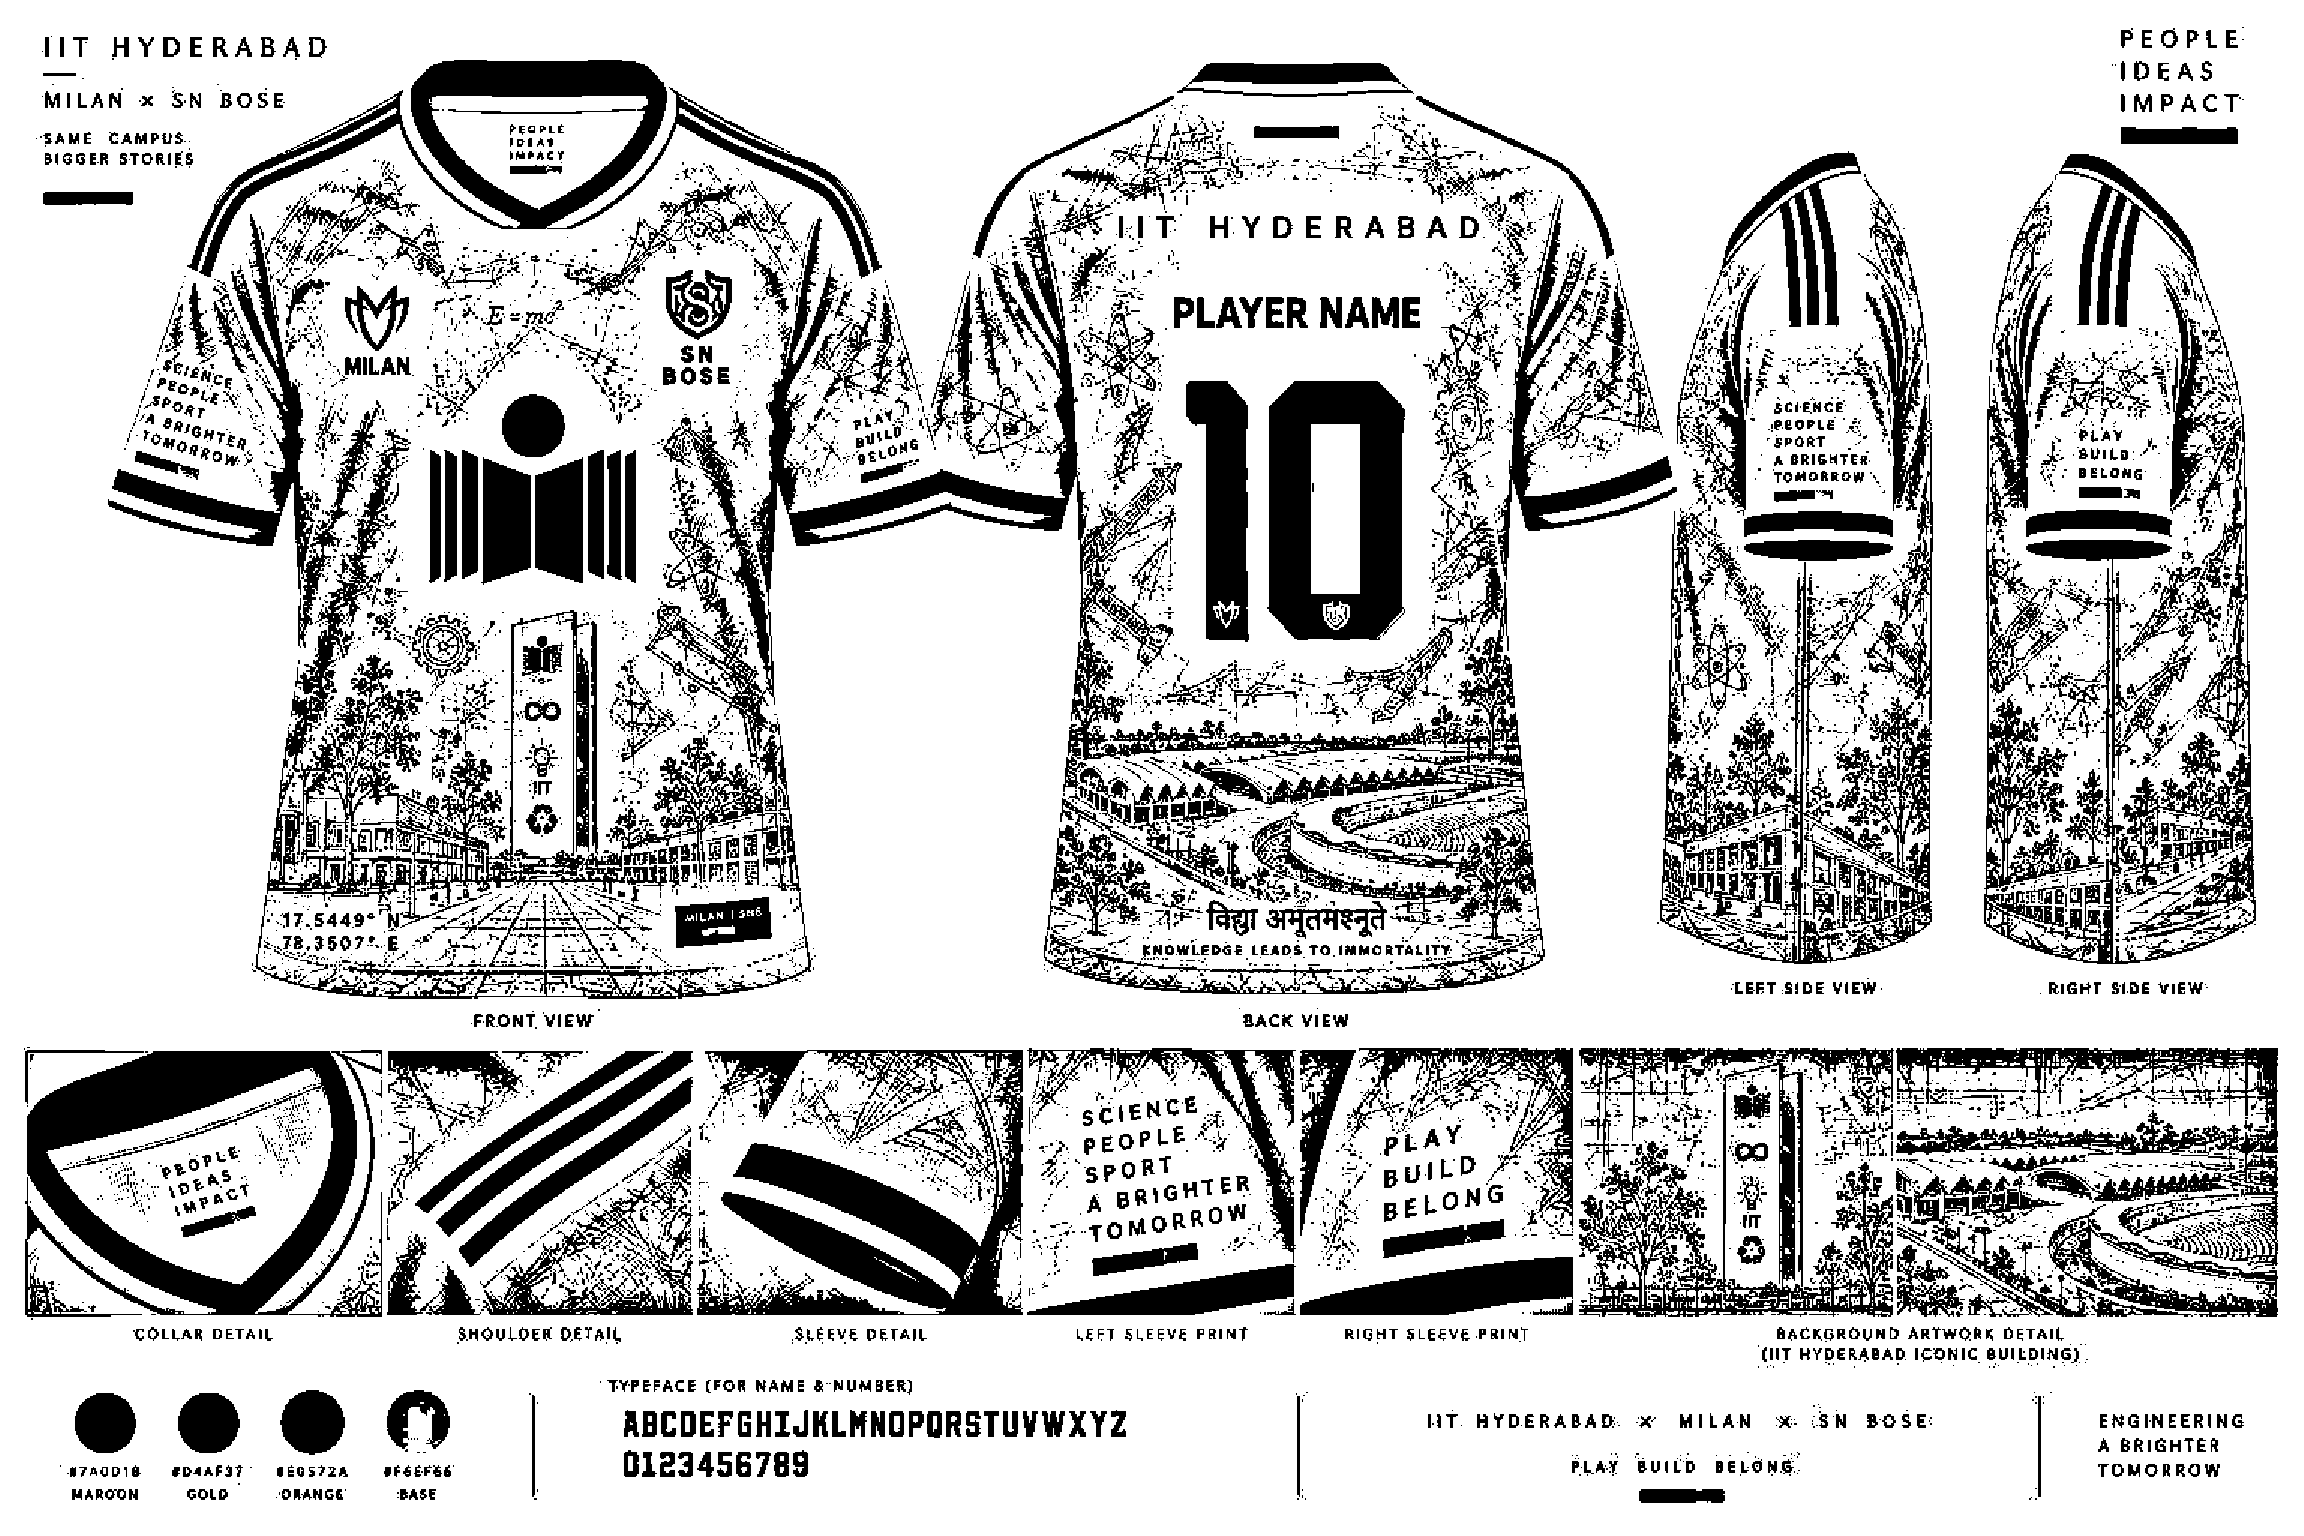
\includegraphics[width=0.5\linewidth]{figs/jersey/gaussian_localized_reference.pdf}
    \caption{Gaussian localized reference with $\sigma=10$ and $C=3$.}
    \label{fig:jersey_gaussian_localized}
\end{figure}

\begin{figure}[H]
    \centering
    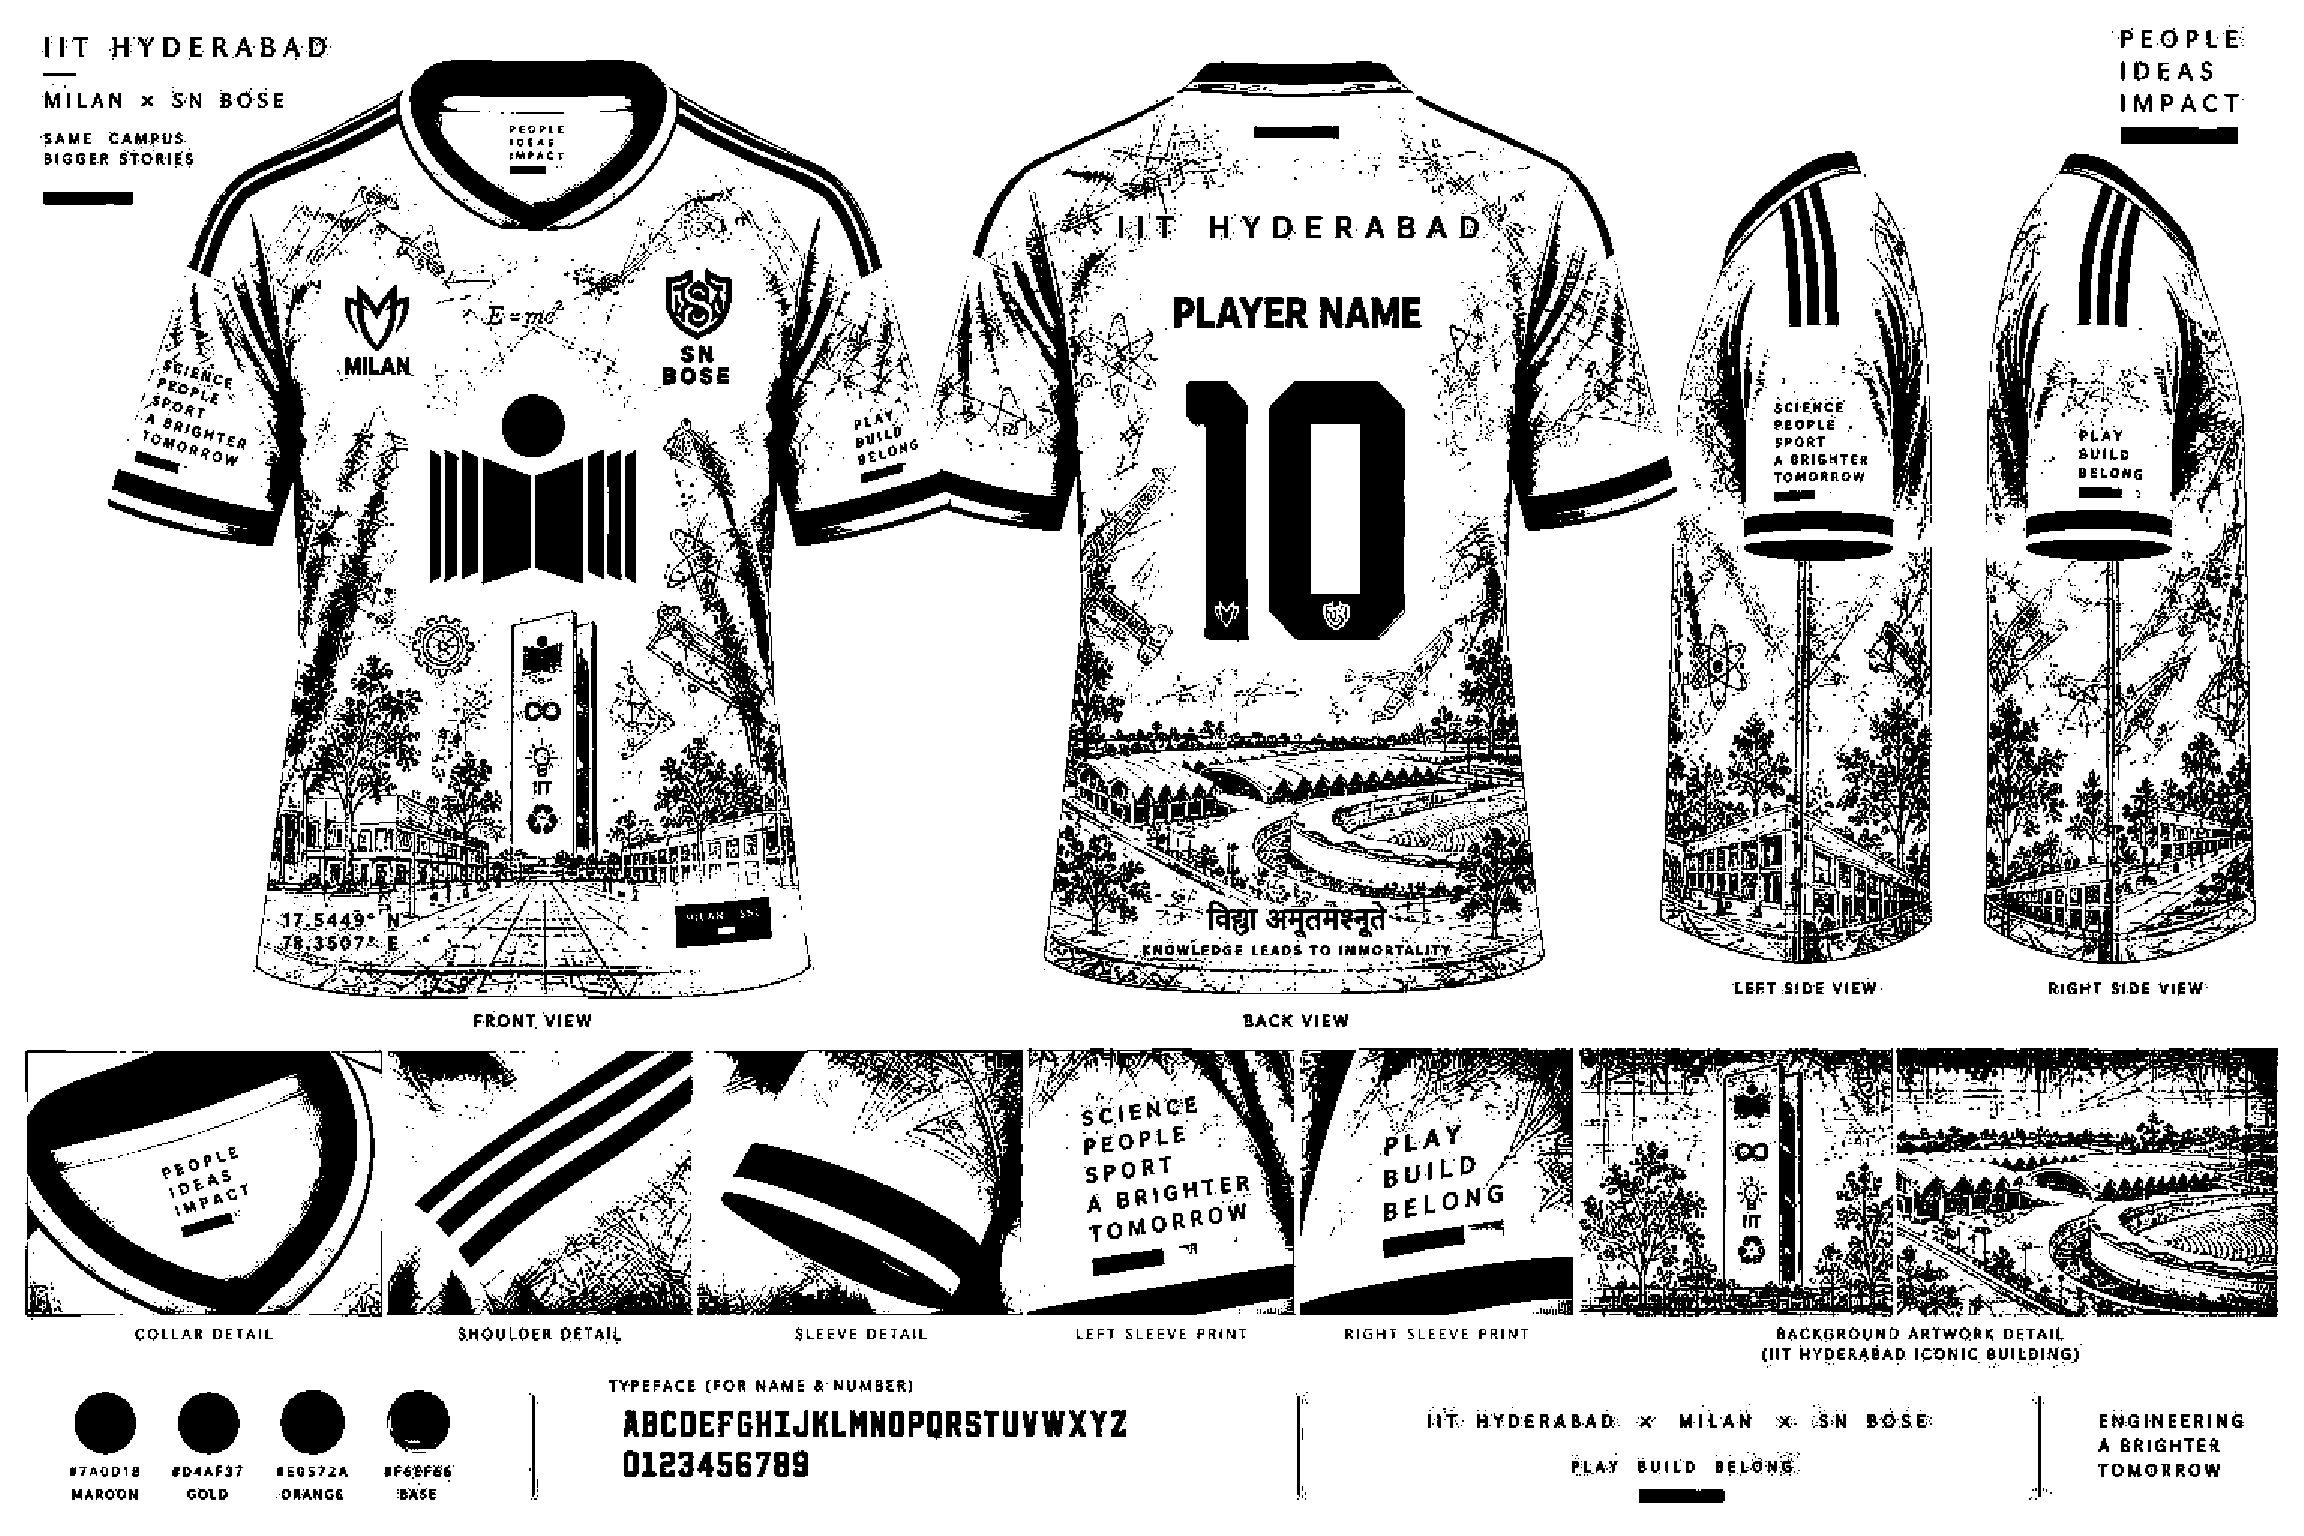
\includegraphics[width=0.5\linewidth]{figs/jersey/gaussian_wide_reference.pdf}
    \caption{Gaussian wide reference with $\sigma=20$ and $C=3$.}
    \label{fig:jersey_gaussian_wide}
\end{figure}
\vspace*{\baselineskip}
\subsection{Program File}

The complete Python code used to generate the grayscale and
black-and-white outputs is:

\begin{lstlisting}[frame=single, basicstyle=\rmfamily, escapeinside={(*@}{@*)}]
(*@\makebox[\dimexpr\linewidth-2\fboxsep-2\fboxrule\relax][c]{codes/image.py}@*)
\end{lstlisting}


\vspace*{5\baselineskip}
\section{\textbf{References}}
\subsection{Reference 1: RGB Image Representation}
ITU-T Recommendation T.871, \textit{JPEG File Interchange Format (JFIF)}.
\url{https://www.itu.int/rec/T-REC-T.871/en}

\subsection{Reference 2: JPEG Image Compression}
ITU-T Recommendation T.81, \textit{Information technology -- Digital compression and coding of continuous-tone still images -- Requirements and guidelines}.
\url{https://www.itu.int/rec/T-REC-T.81/en}

\subsection{Reference 3: Y, Cb and Cr Conversion}
ITU-R Recommendation BT.601, \textit{Studio encoding parameters of digital television for standard 4:3 and wide-screen 16:9 aspect ratios}.
\url{https://www.itu.int/rec/R-REC-BT.601/en}

\subsection{Reference 4: Image Thresholding}
scikit-image Documentation, \textit{Image Thresholding}.
\url{https://scikit-image.org/docs/stable/auto_examples/applications/plot_thresholding_guide.html}

\subsection{Reference 5: Gaussian Filtering}
SciPy Documentation, \textit{Multidimensional Gaussian Filter}.
\url{https://docs.scipy.org/doc/scipy/reference/generated/scipy.ndimage.gaussian_filter.html}


\end{document}
